\documentclass[hidelinks,a4paper,fleqn,oneside]{book}
\usepackage[utf8]{inputenc}
\usepackage[hmargin=2.4cm,vmargin=2.4cm]{geometry}
\usepackage{amsfonts}
\usepackage[makeroom]{cancel}
\usepackage{amsmath,amsthm,amssymb}
\usepackage{polski}
\usepackage{ulem}
\usepackage{makeidx}

\usepackage{minted}

\setminted[python]{
    breaklines=true,
    mathescape=true,
    escapeinside=||,
    encoding=utf8
}

% minted workaround
\makeatletter
\AtBeginEnvironment{minted}{\dontdofcolorbox}
\def\dontdofcolorbox{\renewcommand\fcolorbox[4][]{##4}}
\makeatother

\usepackage{tikz}
\usetikzlibrary{snakes}
\usetikzlibrary{decorations.pathreplacing,decorations}
\usetikzlibrary{patterns}

\setlength{\parindent}{0em}
\setlength{\parskip}{0.4em}

\usepackage{longtable}

\author{wiedza zebrana z wykładów dr Piotra Krzyżanowskiego i materiałów na ważniaku}
\title{Numerki}

\newcommand{\II}{\mathbb{I}}
\newcommand{\RR}{\mathbb{R}}
\newcommand{\EE}{\mathbb{E}}
\newcommand{\CC}{\mathbb{C}}
\newcommand{\ra}{\rightarrow}
\newcommand{\la}{\leftarrow}
\newcommand{\pl}{\parallel}
\newcommand{\eye}{I}

\newcommand{\norm}[1]{\left\lVert#1\right\rVert}

\newtheorem{wniosek}{Wniosek}
\newtheorem{defi}{Definicja}
\newtheorem{fakt}{Fakt}
\newtheorem{lemat}{Lemat}
\newtheorem{twierdz}{Twierdzenie}
\newtheorem{obserw}{Obserwacja}

\usepackage{dirtytalk}

\makeindex
\usepackage[nottoc]{tocbibind}

\begin{document}
\linespread{1.0}
\maketitle

\tableofcontents

\clearpage

\section*{Info na start}

\begin{itemize}
	\item 10p. aktywność na ćwiczeniach (pewnie prace domowe)
	\item 20p. lab
	\item 20p. kolos 23.XI. na wykładzie
	\item 50p. egzamin
\end{itemize}

Ocena: $max(K + L + C + E, 2 \cdot E - 5)$

I termin: $K + L + C > 20p$

G. Stewart ``Afternotes on numerical analysis"

\chapter{Arytmetyka komputerowa}

\section{Wstęp}
\[
	\underbrace{6,63}_{mantysa} \cdot \underbrace{10^{\overbrace{-34}^{\textrm{wykładnik}}}}_{\textrm{rząd wielkości}}
\]

Liczby maszynowe:

$x = (-1)^{\overbrace{s}^{\textrm{znak}}} \cdot \underbrace{m}_{\textrm{mantysa}} \cdot \underbrace{\beta^{\overbrace{e}^{\textrm{wykładnik}}}}_{\textrm{podstawa - u nas 2}}$

$0 \leq m < \beta$

$e - \textrm{wykładnik, liczba całkowita taka, że } 0 > e_{min} \leq e \leq e_{max} > 0$

Charakterystyka zestawu: $(\beta, \underbrace{e_{min}, e_{max}}_{zakres}, \underbrace{p}_{precyzja})$

\textbf{Liczby znormalizowane}\index{liczba znormalizowana}:
\[
	x = (-1)^s \cdot m \cdot 2^e
\]

ale zakładamy, że m jest postaci (a więc $1 \leq m < 2)$
\[
	m = (1.f_1,f_2,f_3,...)
\]

To daje jednoznaczną reprezentację liczb niezerowych. Dodatkowo $f_0$ nie trzeba pamiętać w pamięci komputera.

\section{Standard arytmetyki zmiennopozycyjnej}

$\underbrace{\textrm{IEEE-754}}_{Kahan} \rightarrow \textrm{IEEE-854} \rightarrow \underbrace{\textrm{IEEE-754-R}}_{e_{min} = 1 - e_{max}}$
\index{IEEE-754}
W pamięci komputera przechowujemy:

\begin{tabular}{|c|c|l|l|l|c|c|c|l|c|}
	\hline
	s & \multicolumn{4}{c|}{e + bias} & $f_1$ & $f_2$ & \multicolumn{2}{c|}{...} & $f_{p-1}$ \\ \hline
\end{tabular}


\begin{longtable}[c]{l|l|l|l|l|l|l}
	nazwa               & p   & $e_{min}$ & $e_{max}$ & size & bias  & nazwa IEEE-754-R \\ \hline
	\endfirsthead
	%
	\endhead
	%
	single precision    & 24  & -126      & +127      & 32   & 127   & binary32         \\ \hline
	double precision    & 53  & -1022     & +1023     & 64   & 1023  & binary64         \\ \hline
	double extended     & 64  & -16382    & +16383    & 80   & 16383 &                  \\ \hline
	half precisision    & 11  & -14       & 15        & 16   & 15    & binary16         \\ \hline
	quadruple precision & 113 & -16382    & +16383    & 128  & 16383 & binary128        
\end{longtable}

\begin{tabular}{|c|c|l|l|l|c|c|c|l|c|}
	\hline
	0 & \multicolumn{4}{c|}{0...0} & 0 & 0 & \multicolumn{2}{c|}{...} & 0 \\ \hline
\end{tabular} = $+0.0$

\begin{tabular}{|c|c|l|l|l|c|c|c|l|c|}
	\hline
	1 & \multicolumn{4}{c|}{0...0} & 0 & 0 & \multicolumn{2}{c|}{...} & 0 \\ \hline
\end{tabular} = $-0.0$

\begin{tabular}{|c|c|l|l|l|c|c|c|l|c|}
	\hline
	0 & \multicolumn{4}{c|}{1...1} & 0 & 0 & \multicolumn{2}{c|}{...} & 0 \\ \hline
\end{tabular} = $+\infty$

\begin{tabular}{|c|c|l|l|l|c|c|c|l|c|}
	\hline
	1 & \multicolumn{4}{c|}{1...1} & 0 & 0 & \multicolumn{2}{c|}{...} & 0 \\ \hline
\end{tabular} = $-\infty$

\begin{tabular}{|c|c|l|l|l|c|c|c|l|c|}
	\hline
	0 & \multicolumn{4}{c|}{1...1} & niezero \\ \hline
\end{tabular} = NaN

np. $\frac{0}{0} = \infty - \infty = NaN$

\subsection{Zabawkowy system floating point}

(bez biasu)

$\beta = 2$, $p = 3$, $e_{min} = -1$, $e_{max} = +1$

$x = (1.f_1f_2)_2 \cdot 2^{e}$

\begin{tikzpicture}[snake=zigzag, line before snake = 5mm, line after snake = 5mm]
	% draw horizontal line
	\draw [->] (0,0) -- (16,0);
	
	% draw vertical lines
	\foreach \x in {1, 5, 9, 13}
	\draw (\x cm,6pt) -- (\x cm,-6pt);
	
	\foreach \x in {3, 3.5, 4, 4.5, 6, 7, 8, 11, 15}
	\draw (\x cm,3pt) -- (\x cm,-3pt);
	
	% draw nodes
	\draw (1,0) node[below=6pt] {$ 0 $};
	\draw (3,0) node[below=6pt] {$ \frac{1}{2} $};
	\draw (5,0) node[below=6pt] {$ 1 $};
	\draw (9,0) node[below=6pt] {$ 2 $};
	\draw (13,0) node[below=6pt] {$ 3 $};
\end{tikzpicture}


Aby wypełnić pustkę wokół zera uzupełnia się system o liczby subnormalizowane\index{liczba subnormalizowana}:
\[
	(0.f_1f_2...f_{p-1})_2 \cdot 2^{e_{min}}
\]

Reprezentacja liczb rzeczywistych w arytmetyce fl:
\[
	x \in \mathbb{R} \rightarrow fl(x) : \textrm{numeryczna reprezentacja x (l. maszynowa odpowiadająca x)}
\]

Gdy x - liczba maszynowa, fl(x) = x.

Jeśli nie, to
\[
	fl(x) = \texttt{Round(x)}
\]

Gdzie \texttt{Round(x)} może być wybrany na jeden ze sposobów:

\begin{enumerate}
	\item \texttt{RN(x)} - zaokrąglenie do najbliższej liczby maszynowej (domyślne)
	\item \texttt{RD(x)} - zaokrąglenie w dół (tzn. w stronę $-\infty$)
	\item \texttt{RU(x)} - zaokrąglenie w górę (tzn. w stronę $\infty$)
	\item \texttt{RZ(x)} - zaokrąglenie w stronę zera
\end{enumerate}

Dalej zakładamy, że $fl(x) = \texttt{RN(x)}$. Wtedy łatwo pokazać, że 
\[
	\frac{|fl(x) - x|}{|x|} \leq 2^{-p} = \nu \leftarrow \textrm{ precyzja arytmetyki}
\]

(o ile nie ma underflow/overflow)

Inaczej mówiąc:
\[
	fl(x) = x(1 + \varepsilon), |\varepsilon| \leq \nu
\]

---
\[
	a\ \square\ b\ \textrm{jest równy} fl(a\ \square\ b)\textrm{, gdzie }\square \in \{+, -, \times, :\}
\]

co zapisujemy
\[
	\underbrace{fl(a\ \square\ b)}_{\textrm{wynik w fl}} = \underbrace{fl(a\ \square\ b)}_{\textrm{reprezentacja } a \square b \textrm{ w fl}}
\]

(o ile brak underflow/overfow/NaN)

Ponadto tak też ma być dla $\sqrt{}$ i dla
\[
	\underbrace{FMA(a, b, c)}_{\textrm{fast multiply add}} := a \cdot b + c
\]

$fl(FMA(a, b, c)) = fl(a \cdot b + c)$

\section{Problemy arytmetyki fl}

Źródła błędu algorytmu rozwiązującego zadanie:
\begin{itemize}
	\item reprezentacja danych w fl
	\item reprezentacja wyniku w fl
	\item realizacja algorytmu w fl
\end{itemize}


\subsection{Redukcja cyfr przy odejmowaniu}

Dane: $x, y \in \RR$. Obliczamy
\[
	s := x + y
\]

\begin{enumerate}
	\item Reprezentacja danych: $\tilde{x} = fl(x) = x(1+\varepsilon)$,
	      $\tilde{y} = fl(y) = y(1 + \varepsilon)$
	\item Wykonanie algorytmu
	      \[
	      	\tilde{s} = fl(\tilde{x} + \tilde{y}) = (\tilde{x} + \tilde{y})(1 + \varepsilon)
	      \]
\end{enumerate}

Jaki jest błąd?
\[
	\cfrac{|\tilde{s} - s|}{|s|} = \cfrac{|x + (\varepsilon_x + \varepsilon)\cdot x + y + (\varepsilon_y + \varepsilon)\cdot y + \textrm{małe }\nu^2|}{|x + y|} \leq 2 \cdot \cfrac{|x|+|y|}{|x+y|} \cdot \nu
\]

Zatem

- jeśli $x \simeq -y$, to $2\cfrac{|x|+|y|}{|x+y|} \gg 1$. Czyli błąd względny może być bardzo duży.

- jeśli $x, y$ - tego samego znaku, to $2 \cfrac{|x|+|y|}{|x+y|} = 2 \cfrac{|x+y|}{|x+y|} = 2$. Czyli błąd względny na poziomie $\nu$.

\subsection{Błędy w obliczeniach numerycznych}

Zadanie obliczeniowe: $P: \RR^n \supset D \ra \RR^n$. Mając dane $x \in D$ (dziedzina), wyznaczyć $y = P(x)$.

Dane:

\begin{enumerate}
	\item Dane: $x \in \RR$. Obliczyć $y=\sin(x)$.
	\item Dane: $A \in \RR^{N \times N}$, $x \in \RR^n$. Obliczyć $y = A \cdot b$.
	      $D = \RR^{N \times N} \times R^N$
	\item Dane $A \in \RR^{N \times N}$, $b \in \RR^n$. Obliczyć rozwiązanie układu $Ay = b$. Wtedy $P(x) := A^{-1}x$
	\item Dla danego $F: \RR \ra \RR$ obliczyć $x$, t. że $f(x) = 0$,
	      $P(z) = f^{-1}(z)$, $D = \{0\}$
\end{enumerate}


\section{Numeryczna poprawność}

Pożądane jest, aby algorytm dawał "dobry" wynik zarówno w arytmetyce idealnej, jak i w arytmetyce $fl$. Niestety, jak zobaczymy, nie zawsze jest to możliwe. Nawet jeśli algorytm jest dokładny, to w wyniku jego realizacji w $fl$ możemy otrzymać wynik $fl(ALG(x))$ daleko odbiegający od $P(x)$. W szczególności, prawie zawsze mamy
\[P(x) \neq fl(ALG(x))\]
Zauważmy również, że o ile z reguły znamy dokładne zachowanie się algorytmu w arytmetyce idealnej dla danej informacji, to nie można tego samego powiedzieć o jego zachowaniu się w arytmetyce $fl$. W związku z tym powstaje pytanie, jak kontrolować błąd algorytmów wynikający z błędów zaokrągleń i jakie algorytmy uznamy za te o najwyższej jakości numerycznej.

Istnienie błędów reprezentacji liczb rzeczywistych powoduje, że informacja $y=N(f)$ o danej $f$ nie jest w ogólności reprezentowana dokładnie. Znaczy to, że zamiast na informacji dokładnej, dowolny algorytm będzie operować na informacji nieco zaburzonej $y_\nu$, tzn. zaburzonej na poziomie błędu reprezentacji. Tak samo wynik dawany przez algorytm będzie w ogólności zaburzony na poziomie błędu reprezentacji. W najlepszym więc wypadku wynikiem działania algorytmu w $fl_\nu$ będzie $(\varphi(y_\nu))_\nu$ zamiast $\varphi(y)$. Algorytmy dające tego rodzaju wyniki uznamy za posiadające najlepsze własności numeryczne w arytmetyce $fl$u i nazwiemy numerycznie poprawnymi.

Niech:
\begin{itemize}
    \item $x \in \RR^n$ - dokładna wartość
    \item $\tilde{x} \in \RR^n$ - wartość przybliżona
    \item błąd bezwzględny - $\parallel \tilde{x} - x \parallel$
    \item błąd względny - $\cfrac{\textrm{błąd bezwzględny}}{\parallel x \parallel}$
\end{itemize}
{\centering 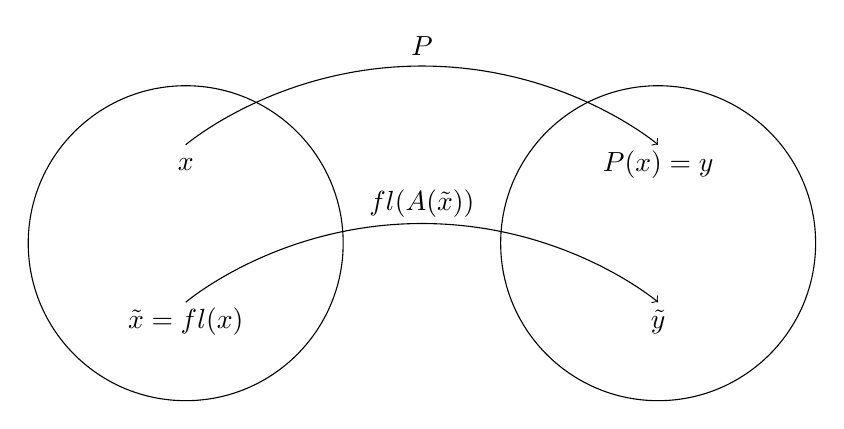
\begin{tikzpicture}
	\draw  (-3,0) ellipse (2 and 2);
	\draw  (3,0) ellipse (2 and 2);
	
	\draw  [->] plot[smooth, tension=1.1] 
	   coordinates {(-3,1.25) (0,2.25) (3,1.25)};
	\node at (-3,1) {$x$};
	\node at (3,1) {$P(x)=y$};
	\node at (0,2.5) {$P$};
	
	\draw  [->] plot[smooth, tension=1.1] 
	   coordinates {(-3,-0.75) (0,0.25) (3,-0.75)};
	\node at (-3,-1) {$\tilde{x} = fl(x)$};
	\node at (3,-1) {$\tilde{y}$};
	\node at (0,0.5) {$fl(A(\tilde{x}))$};
\end{tikzpicture}\par}

{\centering 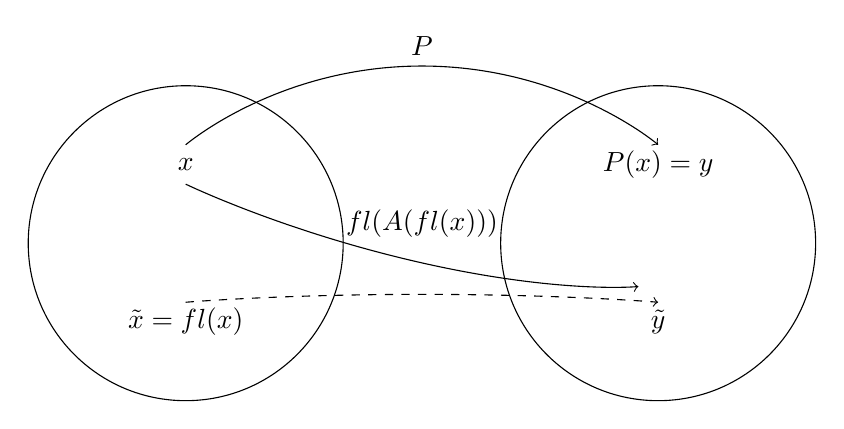
\begin{tikzpicture}
	\draw  (-3,0) ellipse (2 and 2);
	\draw  (3,0) ellipse (2 and 2);
	
	\draw  [->] plot[smooth, tension=1.1] 
	   coordinates {(-3,1.25) (0,2.25) (3,1.25)};
	\node at (-3,1) {$x$};
	\node at (3,1) {$P(x)=y$};
	\node at (0,2.5) {$P$};
	
	\draw  [dashed] [->] plot[smooth, tension=1.1] 
	   coordinates {(-3,-0.75) (0,-0.65) (3,-0.75)};
	\node at (-3,-1) {$\tilde{x} = fl(x)$};
	\node at (3,-1) {$\tilde{y}$};
	\node at (0,0.25) {$fl(A(fl(x)))$};
	
	\draw  [->] plot[smooth, tension=1.1] 
	   coordinates {(-3,0.75) (0,-.25) (2.75,-0.55)};
\end{tikzpicture}\par}

\begin{defi}[Silnie numeryczna poprawność]\index{numeryczna poprawność!silnie NP}
	Algorytm A jest \textbf{silnie numerycznie poprawny (NP)} jeśli $\tilde{y} = P(\tilde{x})$ - dokładny wynik dla trochę zaburzonych danych, gdzie $\frac{\parallel \tilde{x} - x\parallel}{\parallel x \parallel} \leq \underbrace{k}_{\textrm{nieduża stała}} \cdot \nu$
\end{defi}

\begin{defi}[Numeryczna poprawność]\index{numeryczna poprawność}
	Algorytm m jest \textbf{numerycznie poprawny}, jeśli jego wynik możemy zinterpretować jako prawie dokładne rozwiązanie na prawie dokładnych danych.
	
	$c\frac{\parallel \tilde{x} - x \parallel}{\parallel x + y \parallel} \leq k \cdot \nu$ (prawie dokładne dane)
	
	$\cfrac{\parallel \tilde{y} - P(\tilde{x}) \parallel}{\parallel P(x) \parallel} \leq k \cdot \nu$ (prawie dokładny wynik)
	
\end{defi}

{\centering 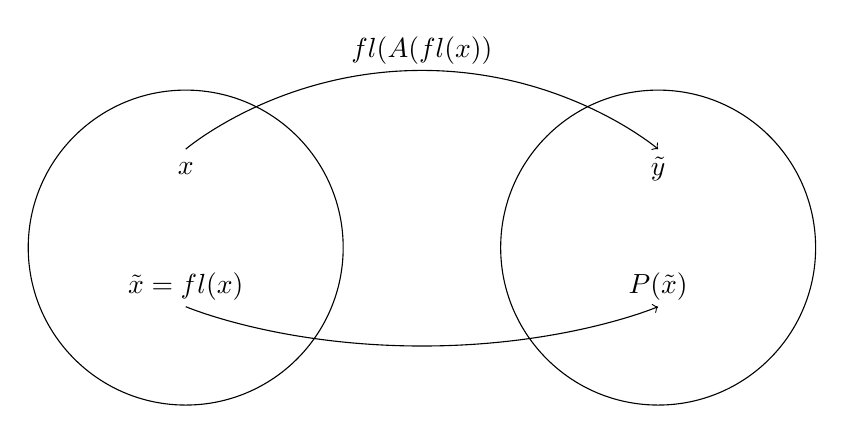
\begin{tikzpicture}
	\draw  (-3,0) ellipse (2 and 2);
	\draw  (3,0) ellipse (2 and 2);
	
	\draw  [->] plot[smooth, tension=1.1] 
	   coordinates {(-3,1.25) (0,2.25) (3,1.25)};
	\node at (-3,1) {$x$};
	\node at (3,1) {$\tilde{y}$};
	\node at (0,2.5) {$fl(A(fl(x))$};
	
	\draw  [->] plot[smooth, tension=1.1] 
	   coordinates {(-3,-0.75) (0,-1.25) (3,-0.75)};
	\node at (-3,-0.5) {$\tilde{x} = fl(x)$};
	\node at (3,-0.5) {$P(\tilde{x})$};
\end{tikzpicture}\par}

\begin{defi}[Polityczna poprawność]\end{defi}

\section{Uwarunkowanie zadania (czułość zadania na zaburzenia)}
Jak zobaczyliśmy w poprzednich przykładach, dane, jakimi dysponujemy wykonując zadanie obliczeniowe, są z natury rzeczy wartościami zaburzonymi. Okazuje się, że powszechna intuicja, że małe zaburzenia danych powinny dawać małe zaburzenia wyniku, nie znajduje potwierdzenia nawet w bardzo prostych przypadkach. Z drugiej strony, umiejętność oceny jakościowego wpływu zaburzenia danych na wynik jest kapitalna w świecie obliczeń numerycznych w ogólności, a w szczególności - inżynierskich.

Pytanie: jak dobrym przybliżeniem $P(x)$ jest y? 

$\cfrac{\norm{P(x) - P(\tilde{x})}}{\norm{P(x)}} = \cfrac{\norm{P(X) < y}}{\norm{P(x)}} \leq ?$

To jest pytanie o czułość zadania P na zaburzenia danych i nie ma nic wspólnego z tym jakiego algorytmu użyjemy.


Zamiast iksa biorę iks zaburzony. Pytanie jaki jest błąd (względny):
\[
	\cfrac{\parallel P(x + \delta) - P(x) \parallel}{\parallel P(x) \parallel} \leq ? \cdot \frac{\norm{\delta}}{\norm{x}}
\]
(błąd względny wyniku vs zaburzenie względne danych)

Lub bezwzględny (błąd bezwzględny wyniku)


\begin{defi}\index{uwarunkowanie}
	Wskaźnik (współczynnik) uwarunkowania zadania P w punkcie x
	\[
		cond_{abs}(P, x) := sup_{\delta\textrm{ dost. małe}}\left(\frac{\norm{P(x + \delta) - P(x)}}{\norm{\delta}}\right)
	\]
	wtedy (dla tych $\delta$):
	\[
		\norm{P(x + \delta) - P(x)} \leq cond_{abs} (P, x) \cdot \norm{\delta}
	\]
	Analogicznie:
	\[
		cond_{rel}(P, x) := sup_{\delta\textrm{ dost. małe}}\left(\frac{\norm{P(x + \delta) - P(x)} \cdot \norm{x}}{\norm{\delta} \cdot \norm{P(x)}}\right)
	\]
	wtedy dla tych $\delta$:
	\[
		\frac{\norm{P(x + \delta) - P(X)}}{\norm{P(x)}} \leq cond_{rel} (P, x) \frac{\norm{\delta}}{\norm{x}}
	\]
	
\end{defi}

\textbf{IDEALIZACJA}: uwarunkowanie w punkcie (tzn. gdy $\delta \ra 0$):
\[\def\arraystretch{3.4}
	\begin{array}{ll}
		cond_{abs}(P, x) & := \lim_{\norm{\delta} \ra 0} \cfrac{\norm{P(x + \delta) - P(x)}}{\norm{\delta}} \\
		cond_{rel}(P, x) & := \lim_{\norm{\delta} \ra 0} \cfrac{\norm{P(x + \delta) - P(x)} \cdot \norm{x}}{\norm{\delta} \cdot \norm{P(x)}} \\ & = cond_{abs} (P, x) \cdot \cfrac{\norm{x}}{\norm{P(x)}}
	\end{array}
\]

\textbf{PRZYKŁAD}:

$P(x) = f(x) \in \RR, x \in R$

$cond_{abs} (P, x) = cond_{abs}(f, x) = \lim_{| \delta | \ra 0} \cfrac{| f(x + \delta) - f(x)|}{| \delta |} = |f'(x)|$

$cond_{rel}(P, x) = \cfrac{|f'(x)| \cdot |x|}{|f(x)|}$

Powiemy, że zadanie P jest źle uwarunkowane w punkcie x, jeśli:
\[
	cond(P, x) \gg 1
\]
Wtedy małe zaburzenie danych może spowodować duży błąd wyniku. W przeciwnym razie mówimy, że zadanie jest dobrze uwarunkowane.

\begin{wniosek} Algorytm NP w zadaniu dobrze uwarunkowanym musi dawać wynik obarczony małym błędem. \end{wniosek}

\section{Numeryczne kryterium NP}\index{numeryczne kryterium NP}

Mamy jakieś $\tilde{x}$ - przybliżone rozwiązanie $Ax = b$. Pytanie czy spełnia równanie:
\[
	(A + \Delta)\tilde{x} = b + \delta
\]

i jak duże jest $\varepsilon$ t. że:
\[
	\frac{\norm{\Delta}}{\norm{A}}, \frac{\norm{\delta}}{\norm{b}} \leq \varepsilon
\]

Odpowiedź: tak, dla pewnych $\Delta$, $\delta$ i 

\[
	\varepsilon = \frac{\norm{b - A\tilde{x}}}{\norm{A} \cdot \norm{\tilde{x}} + \norm{b}} \la \textrm{łatwo obliczyć!}
\]

Przykłady (na uwarunkowanie)

\begin{itemize}
	\item dodawanie $a+b$:
	      \begin{itemize}
	      	\item dobre uwarunkowanie, gdy $a, b$ -  tego samego znaku,
	      	\item źle uwarunkowane, gdy $a \simeq -b$
	      \end{itemize}
	\item układy równań mogą być źle uwarunkowane: np. macierz Hilberta $H_{i,j} = \frac{1}{i+j-1}$
	\item mnożenie, dzielenie, dodawanie są NP (w standardzie IEEE-754) (o ile brak under/overflow)
	\item rozwiązywanie układów trójkątnych standardowym algorytmem jest NP. $\tilde{x}$ spełnia:
	      \[
	      	(U+\Delta)\tilde{x} = b, \cfrac{|\Delta_{i, j}|}{|U_{i, j}|} \leq N \cdot \nu
	      \]
\end{itemize}

\chapter{Układy równań liniowych}

\section{Wprowadzenie}

$x \in \RR^N$

$A \in \RR^{N,N}, \textrm{nieosobliwa}$

$b \in \RR^N$
\[
	A \cdot x = b
\]

\subsection{Proste układy równań}

\subsubsection{Macierze trójkątne}

$
\left\{
\begin{array}{ll}
	a_{11}x_1                                  & = b_1 \implies x_1 = \cfrac{b_1}{a_{11}}                \\
	a_{21}x_1 + a_{22}x_2                      & = b_2 \implies x_2 = \cfrac{1}{a_{22}}(b_2 - a_{11}x_1) \\
	\vdots \\
	a_{m1}x_1 + a_{m2}x_2 + \cdots + a_{mn}x_n & = b_n                                                   
\end{array}
\right.
$

$x_n = \cfrac{1}{a_{nk}}(b_k - \sum_{j=1}^{k-1} a_{kj}x_j)$

Gdy macierz układu ma formę trójkątną, to koszt wyznaczenia rozwiązania:
\[
	\left[
		\begin{array}{ccccc}
			a_{0,0} \\
			a_{0,1} & a_{1,1}  &   & \text{\huge0}\\
			a_{0,2}  & a_{1,2} & a_{2,2} \\
			\vdots  & \vdots & \vdots & \ddots \\
			a_{0,n} & a_{1,n} & \cdots & a_{n-1,n} & a_{n,n} 
		\end{array}
	\right]
	\cdot
	\left [
		\begin{array}{c}
			x_1 \\  \vdots \\  \vdots \\ x_n
		\end{array}
	\right]
	=
	\left [
		\begin{array}{c}
			b_1 \\ \vdots \\ \vdots \\ b_n
		\end{array}
	\right]
\]

to

\begin{align*}
	x_0 & = \frac{b_0}{a_{0,0}}                                & \text{(jedna operacja)}    \\
	x_1 & = \frac{b_1 - a_{0,1} x_0}{a_{1,1}}                  & \text{(trzy operacje)}     \\
	&\vdots \\
	x_n & = \frac{b_n - \sum_{i=0}^{n-1} a_{i,n} x_i}{a_{n,n}} & \text{($2n + 1$ operacji)} 
\end{align*}

Koszt rozwiązania jest następujący:
$1+3+5+...+2(k-1)+... = \sum_{k=1}^{n} 2k - \sum 1 = O(n^2)$

Jest to metoda podstawienia w przód/tył. Rozmiar danych jest rzędu $O(n^2)$, więc widać, że jest to optymalna metoda.

\subsubsection{Macierze ortogonalne}

Gdy mamy macierz ortogonalną, tzn.

$Q^T \cdot Q = I$, gdzie $Q \in \RR^{N, N}$

$\arraycolsep=0.6em\def\arraystretch{1.8}
\left[
	\begin{array}{c}
		\quad q_1^T \quad   \\ \hline
		\quad q_2^T \quad  \\ \hline
		\quad \vdots \quad \\ \hline
		\quad q_n^T \quad  
	\end{array}
\right]
\cdot
\left[
	\begin{array}{c|c|c|c}
		    &     &        &     \\
		q_1 & q_2 & \cdots & q_n \\
		    &     &        &     
	\end{array}
\right]
=
\left[
	\begin{array}{cccc}
		1 &   &        & 0 \\
		  & 1 &        &   \\
		  &   & \ddots &   \\
		0 &   &        & 1 
	\end{array}
\right]	
$

Jej kolumny są wzajemnie prostopadłe o normie euklidesowej równej $1$. Nietrudno zauważyć, że zachodzi też $Q \cdot Q^T = \eye$.

Układ $Q \cdot x = b$ ma rozwiązanie:
\begin{equation}
	\begin{aligned}
		Q \cdot x           & = b           \\
		Q^T \cdot Q \cdot x & = Q^T b       \\
		x                   & = Q^T \cdot b \\
	\end{aligned}
\end{equation}

koszt rozwiązania to koszt wymnożenia macierzy, zatem  $O(n^2)$.


\subsection{W miarę proste układy równań}

\subsubsection{Układ z łatwym blokiem}

Przypuśćmy, że nasz układ jest postaci blokowej

$\arraycolsep=1em\def\arraystretch{2}
\left[
	\begin{array}{c|c}
		A_1 & E \\ \hline
		B   & C 
	\end{array}
\right] \cdot
\left[
	\begin{array}{c}
		x \\ \hline
		y 
	\end{array}
\right] = 
\left[
	\begin{array}{c}
		f \\ \hline
		g 
	\end{array}
\right]
$

gdzie A, B, C, E to macierze, układy z A potrafimy ``łatwo" rozwiązać.
\[
	\left\{ \begin{array}{l}
	A_1x + Ey = f\\
	Bx + Cy = g
	\end{array} \right.
\]

\[
	\left\{ \begin{array}{l}
	A_1x = f - Ey\\
	Bx + Cy = g
	\end{array} \right.
\]

\[
	\left\{ \begin{array}{l}
	x = A_1^{-1}(f - Ey)\\
	Bx + Cy = g
	\end{array} \right.
\]

\[
	B \cdot A_1^{-1} (f - Ey) + Cy = g \implies (C - BA_1^{-1}E)y = g - B\cdot A_1^{-1}f
\]

\textbf{Algorytm}:

\begin{enumerate}
	\item Rozwiąż układ równań $A_1w = f$
	\item Rozwiąż układ $A_1 \cdot G = E$
	\item Rozwiąż $(C-FG)y = y - Fw$ (jeśli potrafisz)
	\item $x = w - Gy$
\end{enumerate}


\subsubsection{Układy ze znanym rozkładem macierzy}

Załóżmy, że $A = B_1 \cdot B_2$, gdzie macierze $B_1$, $B_2$ są "łatwe". Wtedy układ $A\cdot x = b$ też jest łatwy.

$B_1 \cdot \underbrace{ B_2 \cdot x}_{y} = b$

\textbf{Algorytm}:

\begin{enumerate}
	\item Rozwiąż $B_1 y = b$
	\item Rozwiąż $B_2 x = y$
\end{enumerate}

\subsubsection{}

Zauważmy, że na ten algorytm można popatrzeć jak na rozkład na ``łatwiejsze" macierze
\[\arraycolsep=1em\def\arraystretch{2}
	\left[
		\begin{array}{c|c}
			A_1 & E \\ \hline
			F   & C 
		\end{array}
	\right] =
	\left[
		\begin{array}{c|c}
			\eye     & 0 \\ \hline
			F A^{-1} & I 
		\end{array}
	\right]
	\cdot 
	\left[
		\begin{array}{c|c}
			A_1 & E \\ \hline
			0   & S 
		\end{array}
	\right]
\]

Gdzie $S = C - FG = C - FA^{-1}E$


\textbf{Pomysł}: znaleźć rozkład macierzy A na iloczyn macierzy dolnej i górnej trójkątnej.
\[
	A = \underbrace{\left[
			\begin{array}{cc}
				      & 0 \\
				\star &   
			\end{array}
		\right]}_{L} \cdot
	\underbrace{\left[
			\begin{array}{cc}
				  & \star \\
				0 &       
			\end{array}
		\right]}_{U}
\]

Spróbujmy blokowo:
\[\arraycolsep=0.7em\def\arraystretch{1.4}
	\left[
		\begin{array}{c|c}
			A_{11} & A_{12} \\ \hline
			A_{21} & A_{22} 
		\end{array}
	\right] =
	\left[
		\begin{array}{c|c}
			L_{11} & 0      \\ \hline
			L_{21} & L_{22} 
		\end{array}
	\right]
	\cdot 
	\left[
		\begin{array}{c|c}
			U_{11} & U_{12} \\ \hline
			0      & U_{22}
		\end{array}
	\right]
\]

Mnożąc dostajemy:

$
\begin{array}{ll}
	A_{1,1} & = L_{1,1} \cdot U_{1,1}                                                                           \\
	A_{2,1} & = L_{2,1} \cdot U_{1,1} \implies L_{2,1} = A_{2,1}U_{11}^{-1}                                     \\
	A_{1,2} & = L_{1,1} \cdot U_{1,2}  \implies U_{1,2} = L^{-1}_{1,1} A_{1,2}                                  \\
	A_{2,2} & = L_{2,1} \cdot U_{1,2} + L_{1,2} \cdot A_{2,2} \implies A_{22} - L_{2,1}U_{1,2} = L_{2,2}U_{2,2} 
\end{array}
$

Mamy rekurencyjny algorytm rozkładu $LU$, ale w klasycznym przypadku biorąc podział blokowy można uniknąć rekurencji. \index{rozkład!LU}
\[\arraycolsep=0.7em\def\arraystretch{1.4}
	\begin{array}{l}
		\updownarrow 1   \\ \\
		\updownarrow N-1 \\ \ 
	\end{array}
	\left[
		\begin{array}{c|c}
			a_{11} & \quad a_{12}^T \quad \\ \hline & \\
			a_{21} & A_{22}               \\ &
		\end{array}
	\right] =
	\left[
		\begin{array}{c|c}
			q      & \quad 0^T \quad \\ \hline & \\
			l_{21} & L_{22}          \\ &
		\end{array}
	\right]
	\cdot 
	\left[
		\begin{array}{c|c}
			u_{11} & \quad u_{12}^T \quad \\ \hline & \\
			0      & U_{22}               \\ &
		\end{array}
	\right]
\]

$L_{1,1} = 1$, $u_{1,1} = a_{1,1}$

$L_{2,1} = \frac{1}{a_{1,1}} \cdot a_{?}$

$\underbrace{\tilde{A}_{22} - L_{21}U_{12}^T}_{\textrm{wystarczy rozłożyć taką macierz - stąd algorytm iteracyjny}} = L_{22} \cdot U_{22}$


Można na to patrzeć jako na sekwencję przejść A prowadzącą do macierzy U. A to jest tak naprawdę eliminacja Gaussa.

\section{Algorytm eliminacji Gaussa}
\index{eliminacje Gaussa}
Ten algorytm nie zadziała, jeśli w trakcie będziemy dzielić przez 0, np.

$A = \left[
	\begin{array}{cc}
		0 & 1 \\
		1 & 0 
\end{array}\right]$ (nieosobliwa)
    
Aby algorytm eliminacji Gaussa zadziałał zawsze (o ile tylko A - nieosobliwa), uzupełnimy go o procedurę \uwave{wyboru elementu głównego} (osiowania). 

\begin{enumerate}
	\item Szukamy w kolumnie, w której prowadzimy eliminację, elementu o największym module (niezerowy, bo A nieosobliwa)
	\item "Zamieniam"\footnote{Zamiana wierszy - mnożenie macierzy przez macierz permutacji} wiersz, w którym jest znaleziony element z wierszem wyżej 
\end{enumerate}


\begin{wniosek} Algorytm eliminacji Gaussa z wyborem elementu głównego w kolumnie prowadzi do rozkładu
	\[
		P \cdot A = L \cdot U
	\]
	gdzie $P$ to macierz permutacji, $L$ - dolna trójkątna, $U$ - górna trójkątna.
	
\end{wniosek}

Stąd algorytm rozwiązywania układów równań:

\begin{enumerate}
	\item Rozłóż $PA = LU$
	\item Rozwiąż $Ly = Pb$ $\quad\quad O(n^2)$
	\item Rozwiąż $Ux = y$ $\quad\quad O(n^2)$
\end{enumerate}

Koszt rozkładu:

$2*(n-1)^2 + 2(n-2)^2 + ... + 2 + O(n^2) = 2 \cdot \underbrace{((n-1)^2 + (n-2)^2 + ... + 1^2)}_{\frac{1}{3}n^3}$

\subsection{Uwarunkowanie układu równań liniowych}

\index{uwarunkowanie!układu równań liniowych}
$x = A^{-1}b, Ax = b$

$\tilde{x} = A^{-1}(b + \delta) = A\tilde{x} = b + \delta$, $\frac{\norm{x - \tilde{x}}}{\norm{x}} \leq ?$


$\frac{\norm{\delta}}{\norm{b}} \leq \varepsilon$
\[
	\norm{x - \tilde{x}} = \norm{A^{-1}b - A^{-1}(b + \delta)} = \norm{A^{-1}b - A^{-1}b - A^{-1}\delta} = \norm{A^{-1}\delta} \leq \norm{A} \cdot \norm{\delta}
\]

\[
	\frac{\norm{x - \tilde{x}}}{\norm{x}} \leq \frac{\norm{A^{-1}} \cdot \norm{\delta}}{\norm{x}} = \frac{\norm{A^{-1}} \cdot \norm{\delta} \cdot \norm{b}}{\norm{x} \cdot \norm{b}} \leq \frac{\norm{A^{-1}} \cdot \norm{b}}{\norm{x}} \cdot \varepsilon = \frac{\norm{A^{-1}} \cdot \norm{Ax}}{\norm{x}} \cdot \varepsilon \leq \underbrace{\norm{A} \cdot \norm{A^{-1}}}_{cond(A)} \cdot \varepsilon
\]

Wpływ zaburzeń macierzy i prawej strony:

$Ax = b$, $(a + \Delta)\tilde{x} = b + \delta$, gdzie

$\frac{\norm{\Delta}}{\norm{A}} \leq \varepsilon$, $\frac{\delta}{b} \leq \varepsilon$

Okazuje się, że jeśli:
\[
	\varepsilon \norm{A} \cdot \norm{A^{-1}} \leq \frac{1}{2}
\]

to
\[
	\frac{\norm{x - \tilde{x}}}{\norm{x}} \leq 4 \cdot cond(A) \cdot \varepsilon
\]

\begin{proof}

$(A + \Delta)\tilde{x} = Ax + \delta$

stąd

$A(\tilde{x} - x) = \delta - \Delta \tilde{x} = \delta - \Delta(\tilde{x} - x) - \Delta x$

$(A+\Delta)(\tilde{x} - x) = \delta - \Delta \cdot x$

$\norm{\tilde{x} - x} = \norm{(A+\Delta)^{-1}(\delta - \Delta x)} \leq \norm{(A + \Delta)^{-1}} \cdot \norm{\delta - \Delta}$

\end{proof}

\begin{lemat} Jeśli $\norm{B} < 1$, to macierz $I + B$ jest odwracalna oraz
	\[
		\norm{(I + B)^{-1}} \leq \frac{1}{1 - \norm{B}}
	\]
\end{lemat}

\begin{proof}
	Gdyby była osobliwa, to $\exists x \neq 0$
	\[
		(I + B)x = 0
	\]
	\[
		x + Bx = 0
	\]
	$\norm{x} = \norm{-Bx} = \norm{Bx} \leq \norm{B} \cdot \norm{x}$
	\[
		1 \leq \norm{B}
	\]
	sprzeczność.
\end{proof}

\begin{wniosek} Jeśli $A$ jest odwracalna i $\norm{A ^ {-1} \Delta} < 1$, to $(A + \Delta)^{-1}$ istnieje i rzecz jasna
	\[
		\norm{A \cdot \Delta)^{-1}} \leq \frac{\norm{A^{-1}}}{1 - \norm{A^{-1}} \cdot \underbrace{\norm{\Delta}}_{\leq \varepsilon \cdot \norm{A}}}
	\]
	
	$A + \Delta = A(I + A^{-1} \Delta)$
	
	Zatem
	\[
		\norm{\tilde{x} - x} \leq \frac{\norm{A^{-1}}}{1 - \varepsilon \norm{A^{-1}} \cdot \norm{A}} \leq ... \leq \frac{2 \cdot \norm{A^{-1}} \cdot \norm{A}}{1 - \varepsilon \norm{A^{-1}} \cdot \norm{A}} \cdot \norm{x} \cdot \varepsilon
	\]
\end{wniosek}

\begin{fakt} Algorytm rozwiązywania układu $Ax = b \in \RR^n$ przez rozkład LU z wyborem w kolumnie (eliminacja Gaussa z wyborem w kolumnie) produkuje w fl rozwiązanie $\tilde{x}$ takie, że $\tilde{x}$ spełnia (dokładnie) rozwiązanie:
	\[
		(A + \Delta)\tilde{x} = b
	\]
	
	gdzie
	\[
		\frac{\norm{\Delta}_\infty}{\norm{A}_\infty} \leq \underbrace{K}_{\textrm{nieduża stała}} \cdot N^3 \cdot \overbrace{\rho_N}^{\textrm{wskaźnik wzrostu}} \cdot \underbrace{\nu}_{\textrm{precyzja fl}}
	\]
	
	gdzie
	\[
		\rho_N = \frac{max_{i, j, k} |a_{i, j}^{(k)}|}{max_{i, j}|a_{i,j}|}
	\]
\end{fakt}

Niestety $\rho_N \leq 2^{N-1}$ i istnieją macierze, na których jest osiągane. Jednak prawie wszystkie spotykane w życiu macierze mają niewielki wskaźnik wzrostu.

\section{Układy równań z macierzami rozrzedzonymi}

$x \in \RR^N, A \in \RR^{N \times N}$

*) $Ax = b$, $x = ?$. Koszt eliminacji Gaussa dla (*): $O(N^3)$. Często jest tak, że dla $N \gg 1$ wiele elementów $a_{i,j}$ macierzy $A$ będzie zerami. Taką macierz nazywamy macierzą rozrzedzoną (rzadką). Zwykle z macierzach rozrzedzonych liczba niezerowych elementów jest $O(N)$.

\subsection{Formaty przechowywania macierzy rzadkich}

Chcemy przechowywać niezerowe wartości.

\begin{enumerate}
	\item Format współrzędnych - nie ma żadnego uporządkowania
	      %to miala byc tabelka z wykladu, ale nie wyszła
	      %\begin{table}[]
	      %\centering
	      %\begin{tabular}{l|ll|c|ll|}
	      %  & \multicolumn{1}{l|}{0} & .. & k                     & \multicolumn{1}{l|}{} & nnz(A)-1 \\ \cline{2-6} 
	      %I &                        &    & i                     &                       &          \\ \cline{2-6} 
	      %  & \multicolumn{1}{l|}{}  &    & \multicolumn{1}{l|}{} & \multicolumn{1}{l|}{} &          \\ \cline{2-6} 
	      %J &                        &    & j                     &                       &          \\ \cline{2-6} 
	      %  & \multicolumn{1}{l|}{}  &    & \multicolumn{1}{l|}{} & \multicolumn{1}{l|}{} &          \\ \cline{2-6} 
	      %V &                        &    & $a_{i,j}$             &                       &          \\ \cline{2-6} 
	      %\end{tabular}
	      %\end{table}	
	      	
	\item Format CSC/CSR (compressed sparse columns/rows)
	      
	\item Metody bezpośrednie dla macierzy rzadkich:
	      \begin{itemize}
	      	\item zanim rozkład LU (lub $LL^T$)... najpierw permutacje wierszy i kolumn tak, by w czynnikach $LU$ pojawiło się jak najwięcej zer;
	      	      odwracając kolejność wierszy i kolejność kolumn.
	      \end{itemize}
\end{enumerate}


\section{Metody stacjonarne rozwiązywania układów równań liniowych}
\index{metody stacjonarne}
Zamiast poszukiwać dokładnej wartości $x$, takiej że $Ax=b$, znajdźmy jego przybliżenie! Będziemy używać metod iteracyjnych, których podstawowym składnikiem będzie operacja $A \cdot w$, która kosztuje $O(N)$, jeśli $\overbrace{nnz}^{\textrm{non zero}}(A) = O(N)$.


Najprostsze metody (stacjonarne):
\begin{align*}
	A & = M - Z \\
	Ax & = Mx - Zx = b\\
	Mx_{k+1} & = b + Zx_k 
\end{align*}
Zauważamy, że jeśli $x_k \ra x^\star$ to,
\[
	Mx_{k+1} \ra Mx^\star,\quad Zx_k \ra Zx^\star
\]

A więc $x^\star$ musi być rozwiązaniem!

**)
\[
	x_{k+1} = M^{-1}(b + Zx_k)
\]

Będziemy dobierać $M$ tak, by rozwiązanie układu $Mx_{k+1} = \tilde{b}$ było łatwe.

\begin{twierdz}
	Jeśli $\norm{M^{-1}Z} < 1$, to metoda (**) jest zbieżna do rozwiązania $Ax = b$ dla każdego $x_0 \in \RR^N$.
\end{twierdz}


\begin{proof}
  Odejmując stronami $x^\star$ we wzorze na iterację
  \begin{align*}
	x_{k+1} - x^\star & = M^{-1}b + M^{-1}Zx_k - x^\star \\
		& = M^{-1}Ax^\star + M^{-1}Zx_k - x^\star \\
		& = \underbrace{M^{-1}(M-Z)x^\star}_{\eye - M^{-1}Z} + M^{-1}Zx_k - x^\star \\
		& = M^{-1}Zx_k - M^{-1}Zx^\star\\
		& = M^{-1}Z(x_k - x^\star) \\ \\
		\norm{x_{k+1} - x^\star} & = \norm{M^{-1}Z(x_k - x^\star)} \\
		& \leq \norm{M^{-1}Z} \cdot \underbrace{\norm{x_k - x^\star}}_{\gamma < 1} \\ \\
		\norm{x_{k+1} - x^\star} & \leq \underbrace{\gamma^{k+1}}_{gdy\ k \ra \infty, to\ \ra 0} \norm{x_0 - x\star}
		 && \qedhere
  \end{align*}
\end{proof}
	
\begin{twierdz}
	Metoda (**) jest zbieżna do $x^\star$ dla każdego

    $x_0 \in \RR^N \iff \underbrace{\rho}_{\substack{\textrm{promień spektralny: }\\ \rho(B) := max\{| \lambda|: \lambda - \textrm{w.wł B}\}}}(M^{-1}Z) < 1$
\end{twierdz}


Konkretny wybór $M$ jednoznacznie definiuje konkretną metodę. Jej zbieżność może zależeć od własności macierzy A (i samej M).

---

Przykłady metod stacjonarnych (iteracji prostej):
\[
	\left\{ \begin{array}{ll}
	a_{11}x_1^{(k+1)} + a_{12}x_2^{(k)} + ... + a_{1N}x_N^{(k)} & = b_1 \\
	a_{21}x_1^{(k)} + a_{22}x_2^{(k+1)} + ... + a_{2N}x_N^{(k)} & = b_2 \\
	& ... \\
	a_{N1}x_1^{(k)} + a_{N2}x_2^{(k)} + ... + a_{1N}x_N^{(k+1)} & = b_N \\
	\end{array} \right.
\]

\[
	\begin{array}{ll}
		a_{11}x_1^{(k+1)} & = b_1 - a_{12}x_2^{(k)} - ... - a_{1N}x_N^{(k)} \\
		a_{22}x_2^{(k+1)} & = b_2 - \sum_{j\neq 2} a_{2j}x_j^{(k)}          \\
		                  & ...                                             \\
		a_{NN}x_N^{(k+1)} & = b_N - \sum_{j\neq N} a_{Nj}x_N^{(k)}          \\
		M                 & = diag(A) = D                                   
	\end{array}
\]

D - macierz Jacobiego, może być wolno zbieżna.

\begin{twierdz}[o zbieżności macierzy Jacobiego] Niech A ma dominującą przekątną, tzn.
	\[
		|A_{ii}| > \sum_{j \neq i}|a_{ij}| \forall_{i=1..N}
	\]
	wtedy m. Jacobiego jest zbieżna. (dowód był)
\end{twierdz}
 

\subsection{Metoda Gaussa-Seidla} \index{metody stacjonarne!Gaussa-Seidla}
\[
	\begin{array}{ll}
		a_{11}x_1^{(k+1)} & = b_1 - a_{12}x_2^{(k)} - ... - a_{1N}x_N^{(k)}                     \\
		a_{22}x_2^{(k+1)} & = b_2 - \sum_{j > 2} a_{2j}x_j^{(k)} - \sum_{j < 2} a_{2j}x_j^{k+1} \\
		                  & ...                                                                 \\
		a_{ii}x_i^{(k+1)} & = b_i - \sum_{j > i} a_{ij}x_j^{(k)} - \sum_{j < i} a_{ij}x_j^{k+1} \\
		M                 & =                                                                   
	\end{array}
\]
 
Istnieje wiele innych ``prostych" metod iteracyjnych dla układów równań z macierzą rzadką.

$\quad$ \say{Czy można wymyślić nieproste zadanie o iteracji prostej? Można}

\subsection{Metody przestrzeni Kryłowa}\index{metody stacjonarne!przestrzeni Kryłowa}
k - ta iteracja jest zdefinowana jako
\[
	x_k \in x_0 + K_k
\]
gdzie $K_{k, i} = \{r_0, Ar_0, ..., A^{k-1}r_0\}$, gdzie $r_0 = b - Ax_0$.

\begin{itemize}
	\item Metody oparte na minimalizacji błędu
	      \[
	      	x_u \in x_0 + K_i
	      \]
	      oraz $\norm{x_k - x^\star}_B \leq \norm{x - x^\star}_B \forall_{x \in x_0 + K_k}$ 
	\item Metody oparte na minimalizacji residuum:
	      \[
	      	\norm{b - Ax_k}_B \leq \norm{b - Ax}_B \forall_{x \in x_0 + K_k}
	      \]
\end{itemize}
	
\textbf{Przykład}: metoda gradientów sprzężonych (CG):
\index{metody stacjonarne!gradientów sprzężonych (CG)}
Zakładamy, że $A = A^T > 0$. Wyznaczmy $x_k \in x_0 + K_k$ takie, żeby:
\[
	\norm{x_k - x^\star}_A \leq \norm{x - x^\star}_A \forall_{x \in x_0 + K_k}
\]
gdzie $\norm{y}_A^2 := y^T A y$.	
	
\begin{fakt} Metoda CG daje się zaimplementować tak, że koszt jednej iteracji to jedno mnożenie wektora przez A ($O(N)$).
\end{fakt}	

\begin{fakt} W idealnej arytmetyce zbieżność do $x^k$ w co najwyżej N iteracjach.
\end{fakt}	

\begin{fakt} Po k iteracjach błąd szacuje się przez:
	\[
		\norm{x_k - x*} _A \leq 2 \left(\frac{\sqrt{\kappa} - 1}{\sqrt{\kappa} + 1}\right)^k \norm{x_0 - x^k}_A
	\]
	gdzie $\kappa = cond_2(A) = \norm{A} _2 \cdot \norm{A^{-1}}_2 = \cfrac{\lambda_{max}(A)}{\lambda_{min}(A)}$
	
	Dla macierzy niesymetrycznych, nieosobliwych metoda GMRES minimalizuje $\norm{r_k}_2$, dla $x \in x_0 + K_k$.
\end{fakt}

Jak licząc w niższej prezycji uzyskać wynik wyższej precyzji?

\subsection{Iteracyjne poprawianie rozwiązania}

$Ax = b$

Umiemy ``tanio" obliczyć rozwiązanie w niższej prezycji, ale chcemy uzyskać rozwiązanie w wyższej. Pomysł jest następujący: \textbf{Algorytm iteracynego poprawiania}.

$x_0$ - rozwiązanie obliczone w niższej precyzji (dla uproszczenia: w pojedynczej)

$r = b-Ax_0$ - reziduum obliczone w podwójnej prezycji

Gdybym więc rozwiązał układ rozwiązania taki: $Ae = r$, to dostałbym poprawkę, ktora przyłożona do $x_0$ dałaby poprawne rozwiązanie $x = x_0 + e$. Ale poniważ $Ae = r$ policzę w pojedynczej precyzji to policzę to niedokładnie, ale miejmy nadzieję, że to nam i tak poprawi wynik. Zatem teraz w podwónej precyzji policzę $x = x_0 + e$. Mogę tak robić iteracyjnie:

$x_0$ - rozwiązanie w pojedynczej
\begin{minted}[linenos]{python}
for i = 0, 1, 2, ...:
    r = B - |$Ax_i$|     # podwójna
    |$Ae_i$| = r         # pojedyncza
    |$x_{i+1}$| = |$x_i$| + |$e_i$|   # podwójna
\end{minted}


Analizę algorytmu iteracyjnego poprawiania przeprowadzimy w modelowej sytuacji, tzn:
\begin{minted}[linenos]{python}
for i = 0, 1, 2, ...:
    |$r_i = b - Ax_i$|
    |$Ae_n = r_i$|
    |$x_{i+1} = x_i + e_i$|
\end{minted}
Hej, a gdzie tu uproszczenie? Krok 2 i 4 przeprowadzimy dokładnie (jedynie krok 3 w pojedynczym flu). Załóżmy, że nasz algorytm rozwiązywania równań $Ax = b$ w fl jest numerycznie poprawny. To znaczy, że zamiast wyznaczyć dokładną wartość $e_i$, wyznacza jakieś jego przybliżenie $\tilde{e_i}$ takie, że jest ono dokładnym rozwiązaniem zadania zaburzonego:
\[
	(A + H)\tilde{e_i} = r_i \ \ \ \textrm{(dokładnie)}
\]

przy czym $\norm{H} \leq c \norm{A} \cdot \underbrace{\nu}_{\textrm{precyzja arytmetyki pojedynczej prezycji}}$

Niech $x^\star$ będzie rozwiązaniem dokładnym $Ax = b$.

\begin{align*}
	\underbrace{x^\star - x_{n+1}}_{e_{n+1}} & = \underbrace{x^\star - x_n}_{e_n} - \tilde{e_n} \\
	& = e_n - \tilde{e_n} \\
	& = A^{-1}r_n  - (A+H)^{-1}r_n \\
	& = A^{-1}r_n - (I + A^{-1}H)^{-1}A^{-1}r_n \\
	& = (I - (I + \underbrace{A^{-1}H}_{-B})^{-1})A^{-1}r_n \\ \\
	(I - B)^{-1} - I & = B(I - B)^{-1}
\end{align*}
Zatem
\begin{align*}
	\norm{e_{n+1}} & = \norm{(I - (I - B)^{-1})A^{-1} r_n} \\
	& \leq \norm{I - (I - B){-1}} \cdot \norm{\underbrace{A^{-1} r_n}_{e_n}} \\
	& \leq \norm{B} \cdot \norm{(I - B)^{-1}} \cdot \norm{e_n}
\end{align*}

Jeśli $\norm{A^{-1}H} < 1$ to $(I - B)$ - odwracalne i na mocy wcześniejszego lematu:
\[
	\norm{(I - B)^{-1}} \leq \cfrac{1}{1 - \norm{B}}
\]

Zatem
\[
	\norm{e_n} \leq \cfrac{\norm{B}}{\underbrace{1 - \norm{B}}_{\gamma}} \cdot \norm{e_n}
\]

Jeśli $\gamma < 1$, to $\norm{e_n} \ra 0$ (liniowo)!.

Na czym polega ukulele $\norm{B}$ - dostatecznie małe?
\[
	\norm{B} = \norm{A^{-1} H} \leq \norm{A^{-1}} \cdot \norm{H} \leq c \cdot \norm{A^{-1}} \cdot \norm{A} \cdot \nu = c \cdot cond(A) \nu
\]

Jeśli więc $cond(A)$ jest niezbyt duże względem $\cfrac{1}{\nu}$ to algorytm IR (modelowy) jest zbieżny.

\section{Liniowe zadania najmniejszych kwadratów (LZNK)} \index{LZNK}
Zajmiemy się zadaniem wygładzania liniowego, nazywanym też liniowym zadaniem najmniejszych kwadratów. Jest ono uogólnieniem zadania rozwiązywania kwadratowych układów równań liniowych do przypadku, gdy układ jest nadokreślony - to znaczy, jest więcej równań niż niewiadomych. W takim przypadku nie należy liczyć na to, że uda się nam wskazać rozwiązanie spełniające wszystkie równania (jest ich za dużo!), dlatego będziemy szukać rozwiązania $x$, które minimalizuje resztę:
\[\norm{|b-Ax}_2\]
Jest to praktycznie bardzo często pojawiające się zadanie, a autorem pierwszego rozwiązania był nie kto inny jak sam wielki Gauss.

Okazuje się bowiem, że jeśli np. potraktować $b$ jako dane eksperymentalne (obarczone pewnym losowym błędem pomiaru o rozkładzie normalnym), a $x$ - parametrami zależności liniowej dla punktów pomiaru zadanych w macierzy $A$, to $x$ minimalizujący $\norm{b-Ax}_2$ (właśnie w tej normie!) jest jednocześnie najbardziej prawdopodobnym zestawem współczynników tej zależności. W języku statystyki takie zadanie nazywa się zadaniem regresji liniowej i jest w tym kontekście bardzo często znajdowane w najrozmaitszych gałęziach nauki - wszędzie tam, gdzie zachodzi potrzeba dopasowania parametrów liniowego modelu do wyników uzyskanych na drodze eksperymentu.

Stąd zresztą nazwa zadania: wygładzanie liniowe, bo chodzi nam o to, by dopasowując parametry krzywej do wyników eksperymentu, wygładzić ewentualne błędy pomiarowe.

Mamy zatem układ $n$ równań z $m$ niewiadomymi.
\begin{align*}
	a_{11}x_{1} + ... + a_{1, m}x_m & = b_1 \\
	a_{21}x_{1} + ... + a_{2, m}x_m & = b_2 \\
	\vdots & \\
	a_{n1}x_{1} + ... + a_{n, m}x_m & = b_n
\end{align*}
\[
\left[
	\begin{array}{cc}
	 \\
	 \\
	 \quad A 
	 \\
	 \\ &
	\end{array}
\right]
	\cdot
\left[
	\begin{array}{c}
	 \\
	 x
	 \\ \ 
	\end{array}
\right]
=
\left[
	\begin{array}{c}
	 \\
	 \\
	 b
	 \\
	 \\ \ 
	\end{array}
\right]
\]
Chcemy aby residuum było możliwie małe, tj $\norm{b - Ax}_2 \ra \textrm{min}$!

$\sum_{i}(\sum_{j} a_{ij} x_{j} - b_{i})^2 \ra \textrm{min}$!

Jak to rozwiązać? Przyda nam się jeszcze jeden rozkład.

\subsection{Rozkład QR macierzy prostokątnej} \index{rozkład!QR}

Algorytm rozwiązaywania LZNK przez rozkład QR


\texttt{krok 1: Wyznacz rozkład $A = QR$}

\texttt{krok 2: Mnimalizuj }\begin{align*}
\norm{b - Ax}_2^2 &= \norm{b - QRx}^2_2 \\
& = \norm{Q(Q^Tb - Rx)}_2^2 \\
& \stackrel{\norm{Q y}_2 = \norm{y}_2}{=} \norm{Q^Tb - Rx}_2^2 \\
\\
 \norm{Q^Tb - Rx}_2^2 & = \norm{\left[\cfrac{Q_1^Tb}{Q^Tb}\right] - \left[\cfrac{R_1x}{0}\right]}_2^2 \\
 & = \norm{\cfrac{Q_1^Tb - R_1x}{Q^T b}}_2^2 \\
 & = \norm{Q_1^Tb - R_1x}_2^2 + \norm{Q^T b}_2^2
\end{align*}

Rozwiązaniem jest $x \in R^n$, spełniający układ $m$ równań z macierzą trójkątną:
\[
	R_1x = Q_1^Tb
\]
Rozwiązanie to dostajemy kosztem $O(m^2)$. Obliczenie $Q_1^Tb$ kosztuje $O(n \cdot m)$ flopów. \textbf{Uwaga: }rozkład QR można też wykorzystać do rozwiązanie układu $Ax=b$ gdy $A$ jest kwadratowa, nieosobliwa.

\subsubsection{Wyznaczanie rozkładu QR macierzy $A$ metodą Householdera}

\begin{defi}[Przekształcenie (odbicie) Householdera] 
Niech $v \in R^n$. Określamy:
	
	\[
		H := I - \cfrac{2}{\underbrace{\norm{v}_2^2}_{\gamma}}vv^T
	\]
\end{defi}

Zauważmy, że 
\begin{align*}
H^2 & = (I - \gamma vv^T)(I - \gamma vv^T) \\
& = I - \gamma vv^T - \gamma vv^T + \gamma^2v\underbrace{v^Tv}_{\norm{v}}v^T \\
& = I - 2 \cfrac{2}{\norm{v}}v v^T + \cfrac{4}{\norm{v}}  vv^T \norm{v} \\
& = I
\end{align*}

Ponadto $H = H^T$: $(I - \gamma vv^T)^T = I^T - \gamma(vv^T)^T = I - \gamma(v^T)^T \cdot v^T = H = H^T$.

\begin{wniosek}H jest macierzą ortogonalną
	\[
		H = I - \gamma vv^T \la \textrm{odbicie Householdera}
	\]
\end{wniosek}

Wskażemy $H_1$ takie, żeby:
\[
H_1 \cdot \left[ \begin{array}{c}\\ \\ \quad A \quad \\ \\ \ \end{array} \right] = 
\left[ \begin{array}{c|c}\star & \quad \star \quad \\ \hline \\ 0 & \tilde{A}\\ & \\ & \end{array}\right]
\]

W kolejnym kroku znajdziemy $H_2$ takie, że:
\[
H_2 \tilde{A} = \left[ \begin{array}{c|c}\star & \quad  \quad \\  \\ 0 & \star \\ & \\ & \end{array}\right]
\]

Po $m$ krokach:

$H_m \cdots H_3 H_2 (H_1 A) = \left[ \begin{array}{ccc} & & \text{\huge R}_1 \\ \\ \\ \hline \\ & \quad 0 & \end{array}\right]$.

Jak skonstruować $H_1$? $H_1$ musi mieć następującą własność, mianowicie:
\[
	H_1 a = const\ e_1
\]
gdzie $a_1$ to pierwsza kolumna naszej macierzy.

Szukamy więc $v \in R^n$ takie, że:
\[
	\left(I - \cfrac{2}{\norm{v}_2^2 vv^T}\right)a = const\ e_1
\]

$H_1a = a - \cfrac{2}{\norm{v}_2} v v^Ta = a - \cfrac{2v^Ta}{\norm{v}} \cdot v$.

Szukamy $v$ postaci $v = a - c\cdot e_1$.

Ponieważ $\norm{Ha}_2^2 = \norm{a}^2_2 = c^2 \norm{e_1}^2_2 = c^2$

to $c = \pm \norm{a} ^2_2$.


Zatem $H = I - \cfrac{2}{\norm{v}_2^2} vv^T$, gdzie $v = a \pm \norm{a}_2^2 \cdot e_1$ jest poszukiwanym przekształceniem.

\textbf{Jaki znak wybrać?} Zgodny ze znakiem $a_1$, aby uniknąć (...)?

W praktyce nigdy nie obliczamy jawnie macierzy Q mnożąc przez siebie macierze $H_1, ..., H_n$. Jedyne co potrzebujemy, to mnożenie przez Q (lub $Q^T$) jakiegoś wektora:
\[
	Q \cdot z = H_1(H_2(...(H_{n-1}z)))
\]

$y = Qz$ obliczamy:
\begin{minted}[linenos]{python}
y = z
for i = m - 1 downto 1:
    y = |$H_i$|y
\end{minted}

Jak tanio mnożyć $H_i y$?
\[
	H_i y = (I - \gamma vv^T)y = y - \gamma v^Tyv
\]

koszt O(n).
 \index{metoda Householdera}
Koszt rozkładu QR metodą Householdera. Trzeba rozłożyć macierz $n \times n$ przy użyciu tej metody
\[
	\underbrace{T(n, n)}_{\textrm{koszt rozkładu QR macierzy }n \times n} = T(n-1, n-1) + \underbrace{\textrm{koszt wyznaczenia v}}_{O(n)} + \underbrace{\textrm{koszt update (HA)}}_{4(n+1)n flopów?}
\]

Po rachunkach $T(n, m) = 2m^2n - \cfrac{2}{3}m^3$ (plus wyrazy niższego rzędu). W szczególności gdy $m = n$, to $T(n, m) = \cfrac{4}{3} n^3$.

\subsection{Rozkład SVD macierzy} \index{rozkład!SVD}
% przypomnienie z zeszłego tygodnia
%LZNK: znaleźć $x \in \RR^m$:
%
%\[
%	\norm{b - Ax}_2 \ra min!
%\]
%
%$A \in \RR^{n \times m}$, $n \geq m$, $rank(A) = m$ (macierz pełnego rzędu).

%Rozwiązanie można otrzymać przez rozkład QR macierzy A.

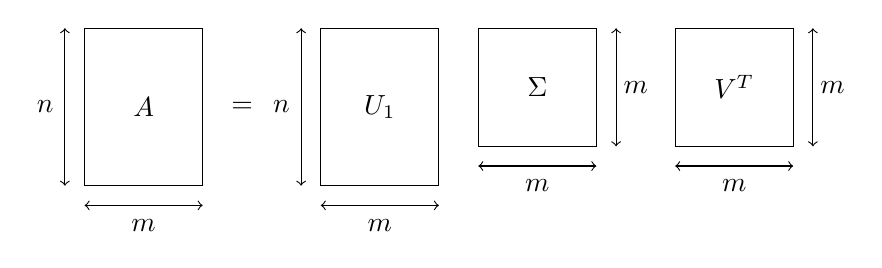
\begin{tikzpicture}
	\draw (0,0) rectangle (1.5, 2);
	\node at (0,0) {};
	\draw [<->] (-0.25,2) -- (-0.25,0);
	\draw [<->] (0,-0.25) -- (1.5,-0.25);
	\node at (2,1) {=};
	\draw (3,0) rectangle (4.5,2);
	\draw [<->](2.75,2) -- (2.75,0);
	\draw [<->] (3,-0.25) -- (4.5,-0.25);
	\draw (5,2) rectangle (6.5,0.5);
	\draw (7.5,2) rectangle (9,0.5);
	\draw [<->] (5,0.25) -- (6.5,0.25);
	\draw [<->]  (6.75,2) -- (6.75,0.5);
	\draw [<->] (7.5,0.25) -- (9,0.25);
	\draw [<->]  (9.25,2) -- (9.25,0.5);
	\node at (0.75,1) {$A$};
	\node at (3.75,1) {$U_1$};
	\node at (5.75,1.25) {$\Sigma$};
	\node at (8.25,1.25) {$V^T$};
	\node at (-0.5,1) {$n$};
	\node at (0.75,-0.5) {$m$};
	
	\node at (2.5,1) {$n$};
	\node at (3.75,-0.5) {$m$};
	\node at (5.75,0) {$m$};
	\node at (7,1.25) {$m$};
	\node at (8.25,0) {$m$};
	\node at (9.5,1.25) {$m$};
\end{tikzpicture}
\[
	A = U_1 \cdot \Sigma_1 \cdot V^T 
\]

Dla każdej macierzy $A \in \RR^{n, m}$ istnieje rozkład:
\begin{itemize}
  \item $U_1^TU_1 = \eye$ (kolumny $U_1$ są ortogonalne)
  \item $V^TV = I$
\end{itemize}
\[
\Sigma_1 = \left[\begin{array}{cccc} \sigma_1 & & & \text{\huge 0} \\
 & \sigma_2 & & \\ & & \ddots & \\ \text{\huge 0} & & & \sigma_n \end{array}\right]
\]

$\sigma _{i}$ - nieujemne wartości szczególne (osobliwe) macierzy A, uporządkowane nierosnąco ($\sigma_{i} \geq 0$).

kolumny $U_1$ - lewe wektory szczególne

kolumny $V$ - prawe wektory szczególne

\textbf{Wariant ``pełny" rozkładu SVD:}

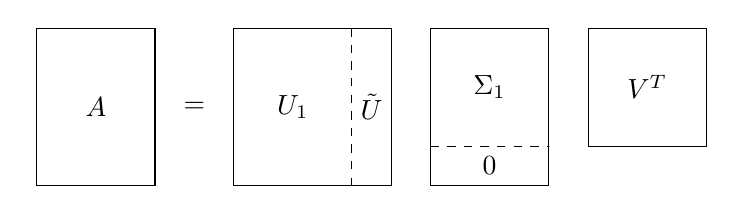
\begin{tikzpicture}
	\draw  (0,0) rectangle (1.5, 2);
	\node at (0,0) {};
	\node at (2,1) {=};
	\draw  (2.5,0) rectangle (4.5,2);
	\draw  (5,2) rectangle (6.5,0);
	\draw  (7,2) rectangle (8.5,0.5);
	\node at (0.75,1) {$A$};
	\node at (3.25,1) {$U_1$};
	\node at (5.75,1.25) {$\Sigma_1$};
	\node at (7.75,1.25) {$V^T$};
	\draw [dashed] (5,0.5) -- (6.5,0.5);
	\draw [dashed] (4,2) -- (4,0);
	\node at (5.75,0.25) {$0$};
	\node at (4.25,1) {$\tilde{U}$};
\end{tikzpicture}

\begin{fakt} $\ $ %todo usunąć ten hack na nową linjkę :D
	\begin{enumerate}
		\item Jeśli $A=A^T$, to oczywście ma rozkład $A = U \cdot \Lambda \cdot U^T$, gdzie kolumny $U$ to wartości własne A, $\Delta = \begin{bmatrix}
		      \lambda_1 & 0 & 0\\ 
		      0 & \ddots & 0\\ 
		      0 & 0 & \lambda_n 
		\end{bmatrix}$, gdzie $\lambda_i$ - wartość własna A.
		
		Wtedy SVD dla A to:
		$A = U\Sigma V^T$, gdzie $\sigma_i = |\lambda_i|$, $v_i = sign(\lambda_i)u_i$
		 			
		\item Wartość własna $A^TA$ to $\sigma_i^2$.
		       			
	      \begin{proof}
	       	$A^TA = (U_1\Sigma V^T)^T(U_1 \Sigma_1 V^T) = V \Sigma_1 \underbrace{U_1^T U_1 \Sigma_1 V^T}_{I} = V \Sigma_1^2V^T$, $\Sigma_1^2 = \begin{bmatrix}
		      \lambda_1^2 & 0 & 0\\ 
		      0 & \ddots^2 & 0\\ 
		      0 & 0 & \lambda_n^2 
			\end{bmatrix}$.
		\end{proof}
				
		\item $AA^T$ jej wartość własna to $\sigma_1^2, ..., \sigma_m^2$ i $(n-m)$ zer.
		      Dowód: analogicnzie jak 2.
		      		
		\item Jeśli $A$ - pełnego rzędu, to rozwiązaniem LZNK $\norm{b - AX}_2 \ra min!$ jest $x = V\Sigma_1^{-1} U_1^Tb$.
		      		
		      \begin{proof}
		      \[
		      	\norm{b - U\Sigma V^Tx} _2 ^2 = \norm{U(U^Tb - \Sigma V^Tx)}_2^2 = \norm{U^Tb - \Sigma V^Tx}_2^2 =
		      	\]
		      	
		      	\[\arraycolsep=1em\def\arraystretch{2} = \norm{\left[\begin{array}{c}
		      	U_1^Tb\\ 
		      	\hline
		      	\tilde{U}^Tb
		      	\end{array}\right] - \left[\begin{array}{c}\Sigma_1V^Tx\\ \hline 0 \end{array}\right]}_2^2 = \norm{\left[\begin{array}{c}U_1^Tb - \Sigma_1V^Tx\\ \hline \tilde{U}^Tb \end{array}\right]}_2^2 =\norm{U_1^Tb - \Sigma_1V^Tx\norm{_2^2 +} \tilde{U}^Tb}_2^2
		      \]
		      
		      x spełniający równanie:
		      \[
		      	\Sigma_1V^Tx = U_1^Tb
		      \]
		      
		      zeruje pierwszy składnik (czyli jak rozwiązanie LZNK)
		      \end{proof}
	\end{enumerate}
\end{fakt}

\subsection{Nieregularne zadanie najmniejszych kwadratów}

Niech $A \in \RR^{m \times n}$, $n \geq m$, ale $rank(A) < m$.

Wtedy LZNK ma niejednoznaczne rozwiązanie.

Jeśli x minializuje $\norm{b - Ax}_2$, to $x+v$ też, o ile $v \in ker(A)$:
\[
	\norm{b - A(x + v)}_2 = \norm{b - Ax - \underbrace{Av}_{=0}}_2 = \norm{b - Ax}_2
\]

Dodając do zadania dodatkowy warunek, że $x$ ma mieć najmniejszą normę $\norm{\cdot}_2$ wśród wszystkich $x$ minimalizujących $\norm{b - Ax}_2$, dostajemy zadanie jednoznaczne: można je rozwiązać, korzystając z SVD!

Ponieważ A jest rzędu $k<m$, to 

\[
	\Sigma_1 = \left[ \begin{array}{ccc|ccc}
		\sigma_1 &  &  &  &  & \\ 
		&  \ddots &  &  & 0  & \\ 
		&  & \sigma_k  &  &  & \\ 
		\hline
		&  & &  0 &  & \\ 
		&  0 &  &  & \ddots & \\ 
		&  &  &  &  & 0
	\end{array} \right]
\]
$\sigma_1 \geq \cdots \geq \sigma_k > 0$.

Zatem
\[\arraycolsep=1em\def\arraystretch{2}
	\left[\begin{array}{c} \\ A \\ \ \end{array}\right] =
	\left[\begin{array}{c|c|c} & &\ \\ \tilde{U}_1 & \hat{U}_1 & \tilde{U} \\ & & \ \end{array}\right] \cdot \left[ \begin{array}{c} \begin{array}{c|c} \tilde{\Sigma}_1 & 0 \\ \hline 0 & 0 \end{array} \\ \hline 0\end{array}\right] \cdot \left[ \begin{array}{c} \tilde{V}_1^t \\ \hline \tilde{V}_2^T \end{array}\right] = \tilde{U}_1 \tilde{\Sigma}_1 \tilde{V}_1^T
\]

Postępując analogicznie jak w 4.
\[\arraycolsep=1em\def\arraystretch{2}
\norm{b - Ax}_2^2 = \norm{\left[ \begin{array}{c}
\tilde{U}_1^T \\ \hline
\hat{U}_1^T \\ \hline
\tilde{U}^T 
\end{array}\right] (b - \tilde{U}_1 \tilde{\Sigma}_1 \tilde{V}_1^Tx)}_2^2 = \norm{\left[\begin{array}{c}
\tilde{U}_1^Tb - \tilde{\Sigma}_1\tilde{V}_1^Tx \\ \hline
\hat{U}_1^T b\\ \hline
\tilde{U}^T b 
\end{array}\right]}_2^2 = 
\norm{\tilde{U}_1^Tb - \tilde{\Sigma}_1\tilde{V}_1^Tx}_2^2 +  \norm{\hat{U}_1^Tb}_2^2 + {\hat{U}^Tb}_2^2
\]

Minimum tego wyrażenia dla $x = \tilde{V}_1\tilde{\Sigma}_1^{-1} \tilde{U}_1^Tb$.

Inne rozwiązania są postaci $x+v$, gdzie $v \in ker(A)$. Ponieważ $v \in ker(A)$ jest postaci $v = \tilde{V}_2 \cdot z$ dla pewnego z.

$\norm{x + v}_2^2 = \norm{x}_2^2 + \norm{v}_2^2$, gdyż $x \bot v$

$x^Tv = (\tilde{V_1} \cdot cos)^T) (\tilde{V}_2z) = cos^T \cdot \underbrace{\tilde{V}_1^T\tilde{V}_2}_{=0}\cdot z = 0$, więc $\norm{x + v}_2$ najmniejsza gdy $v = 0$.

\subsection{Uwarunkowanie LZNK}
\index{uwarunkowanie!LZNK}
$A \in \RR^{n,m}$, $n \gg m$, $rank(A) = m$, $r$ - rozwiązanie LZNK $\norm{b - Ax}_2 \ra min!$

Rozważmy zadanie zaburzone
\[\norm{\tilde{b} - \tilde{A}\tilde{x}}_2 \ra min\]

Załóżmy, że
\[
	\varepsilon := max \left\{ \cfrac{\norm{A - \tilde{A}}_2}{\norm{A} _2}, \cfrac{\norm{b - \tilde{b}}_2}{\norm{b}_2} \right\}
\]

jest na tyle małe, że $cond_2(A) \cdot \varepsilon < 1$, gdzie $cond_2(A) := \cfrac{\sigma_{max}(A)}{\sigma_{min}(A)}$.

Wtedy zadanie zaburzone ma jednoznaczne rozwiązanie oraz $cond_{LZNK}(A, b)$:
\[
	\cfrac{\norm{x - \tilde{x}}_2}{\norm{x}_2} \leq \varepsilon \cdot \underbrace{\left[ \cfrac{2 cond_2(A)}{\cos{\Theta}} + \tan{\Theta}(cond_2(A))^2 \right]}_{cond_{LZNK}(A, b)} + O(\varepsilon^2)
\]

gdzie $\sin{\Theta} = \cfrac{\norm{b - Ax}_2}{\norm{b}_2}$

Zatem:

\begin{enumerate}
	\item $\sin\Theta \simeq$ (tzn. residuum jest małe), wtedy $cond_{LZNK}(A, b) \simeq K cond_2(A)$.
	      	
	\item $\sin\Theta \simeq 1$ (tzn. x jest bliskie zera i duże residuuum!), wtedy $cond_{LZNK}(A, b)\gg 1$ nawet jeśli $cond_2(A) \simeq 1$
	      	
	\item wpp. $cond_{LZNK} \simeq K \cdot cond_2^2(A)$
\end{enumerate}

\section{Zagadnienie własne}
Jednym z podstawowych problemów algebry liniowej jest rozwiązanie zadania własnego, tzn. określeni wartości własnych $\lambda_k$ i wektorów własnych $v$ ($\neq 0$), takich że $Av_k = \lambda_k v_k$. Jeśli $A = A^T$, to wszystkie wartości własne i wektory własne są rzeczywiste i tworzą bazę ortogonalną:
\[
	Q^TAQ = \Lambda = \left[\begin{array}{ccc}
	\lambda_1 &  & \\ 
	&  \ddots & \\ 
	&  & \lambda_n
	\end{array}\right]
\]

gdzie
\[
	Q = \left[ \begin{array}{c|c|c|c} & & & \\ v_1 & v_2 & \cdots & v_n \\ & & & \end{array} \right]
\]

gdzie $Q^TQ = I$.

Zadanie wyznaczania wartości własnych i wektorów własnych macierzy ma bardzo szerokie zastosowania w tak odległych od siebie dziedzinach, jak np. analiza odporności konstrukcji mechanicznych (wieżowce, mosty, wagony kolejowe) na wibracje, czy też rankingowanie stron internetowych w wyszukiwarce Google. Typowe zadania obliczeniowe:

\begin{itemize}
	\item znaleźć ekstremalne wartości własne (lub wektory własne im odpowiadające)
	\item znaleźć wartości własne bliskiej zadanej liczbie (lub ...)
	\item znaleźć wszystkie wartości własne (i wektory).
\end{itemize}

\subsection{Metoda potęgowa}
\index{metoda potęgowa}
Czyli wyznaczanie wektora własnego odpowiadające dominującej wartości własnej

Niech wartości własne A spełniają:
\[
	|\lambda_1| \underbrace{>}_{\textrm{tak, tu ostra}} |\lambda_2| \geq |\lambda_3| \geq \cdots \geq |\lambda_n|
\]

Algorytm:
\begin{minted}[linenos]{python}
for k = 0, 1, 2, ...:
    |$x_{k+1}$| = A * |$x_k$|
    |$x_{k+1} = \frac{x_{k+1}}{\norm{x_{k+1}}_2^2}$|
\end{minted}
Działanie tej metody przeanalizujemy dla A, która jet diagonalizowalna:
\[
	X^{-1} A X = \Lambda = \begin{bmatrix} \lambda_1 &  & \\  &  \ddots & \\ &  & \lambda_n \end{bmatrix}
\]
Innymi słowy:
\[
	AX = X \Lambda
\]
czyli kolumny $v_i$, macierzy X:
 
$X = \left[ \begin{array}{c|c|c|c} &&& \\ v_1 & v_2 & \cdots & v_n \\ &&& \end{array} \right]$ są wektorami własnymi odpowiadającymi $\lambda_i$.
 
Zapisując $x_0 = \sum_{i=1}^{n} \alpha_i v_i$ mamy kolejno:
\begin{align*}
	x_1 & = A \cdot x_0 = A \sum \alpha_iv_i = \sum \alpha_i Av_i = \sum \alpha_i \lambda_i v_i \\
	x_2 & = Ax_1 = A(\sum(\alpha_i\lambda_i)\cdot v_i) = \sum \alpha_i \lambda_i^2 v_i \\
	& \vdots \\
	x_k & = \sum \alpha_i \lambda^k v_i \\ & = \lambda_1^k\left(\alpha_1 v_1 + \alpha_2\underbrace{(\cfrac{\lambda_2}{\lambda_1})^k}_{| \cdots | < 1 \ra 0} v_2 + \cdots + \alpha_n \underbrace{(\cfrac{\lambda_n}{\lambda_1})^k}_{| \cdot | < 1 \ra 0} \cdot v_n\right)
\end{align*}
 
Szybkość zbieżności $x_k$ do kierunku wektora $v_1$ jest proporcjonalna do $\left| \cfrac{\lambda_2}{\lambda_1} \right| < 1$.
 
% powtorzenie wykladu
%Zadanie własne $A \in \RR^{N\times N}$:
%
%\[
%	(\lambda, x) \in \CC \times \CC^N \quad Ax = \lambda \cdot x
%\]

%Co warto zauważyć:

\begin{fakt}
	Jeśli $\lambda$ - w. własna macierzy A, to $(\lambda - \nu)$ - w. własny macierzy $(A - \nu I)$
	\[
		(A - \nu I)v \overbrace{=}^{v\textrm{ - wektor własny odpowiadający }\lambda} = Av - \lambda v = \lambda v - \nu v = (\lambda - \nu)v
	\]
\end{fakt} 

\begin{fakt} Jeśli $\lambda$ - wartość własna A oraz A - nieosobliwa, to $\frac{1}{\lambda}$ jest wartością własną $A^{-1}$.
	\begin{equation}
		\begin{aligned}
			A^{-1}| Av           & = \lambda v                                  \\
			v                    & = A^{-1}(\lambda v) = \lambda \cdot A^{-1} v \\
			\cfrac{1}{\lambda} v & = A^{-1}v                                    
		\end{aligned}
	\end{equation}
\end{fakt}

\begin{fakt} Jeśli $\lambda$ - wartość własna A oraz $(A - \nu I)$ - nieosobliwa, to $\frac{1}{\lambda - \nu}$ jest wartością własną $(A - \nu I)^{-1}$
\end{fakt}

\begin{wniosek} Metoda potęgowa zastosowana do $(A - \nu I)^{-1}$ będzie zbieżna do wartości własnej A, $\lambda_i$, najbliższej $\nu$ (jeśli taka jedyna $\lambda_i$ istnieje). Rzeczywiście, wartość własna $(A - \nu I)^{-1}$ to $\cfrac{1}{\lambda - \nu}$, jeśli zachodzi $\cfrac{1}{|\lambda_i - \nu|} > \cfrac{1}{|\lambda_j - \nu|}$ dla $j \neq i$, to $\cfrac{1}{|\lambda_i - \nu|}$ jest dominująca.
\end{wniosek}

\subsection{Odwrotna metoda potęgowa}
\index{metoda potęgowa!odwrotna}
\begin{minted}[linenos]{python}
for k = 0, 1, 2, ...
    |$x_{k+1}$| = |$(A - \nu I)^{-1}\cdot x_k$|
    |$x_{k+1}$| = |$\frac{x_{k+1}}{\norm{x_{k+1}}}$|
\end{minted}
Ten algorytm w praktyce oczywiście implementujemy inaczej.

$O(N^3) \ra $ Rozłóż macierz na czynniki, np. $P(A-\nu I) = LU$ (albo $A - \nu I = QR$)
\begin{minted}[linenos]{python}
for k = 0, 1, 2, ...
   rozwiąż układ |$Ly = (Px_k)$|         # O(|$n^2$|)
   rozwiąż układ |$U x_{k+1} = y$|          # O(|$n^2$|)
   |$x_{k+1} = \frac{x_{k+1}}{\norm{x_{k+1}}}$|
\end{minted}
Znając przybliżenie $x_k$ wektora własnego, możemy wykonać najlepsze (w sensie średniokwadratowym) przybliżenie wartości własnej:
\[
	\lambda_k = \underbrace{\cfrac{x^T_k A x_k}{x_k^T x_k}}_{\textrm{iloraz Rayleigh}}
\]

(gdy $x_k \in \CC^N$, $\cfrac{x_k^H A x_k}{x_k^Hx_k}$)

Gdy $x_k = v$: $\cfrac{v^TAv}{v^Tv} = \cfrac{v^T \lambda v}{v^T v} = \lambda \cdot \cfrac{v^T v}{v^T v} = \lambda$


\textbf{Metoda Rayleigh:}
\index{metoda Rayleigh}
for k = 0, 1, 2...

Rozwiąż $(A - \nu_k I)x_{k+1} = x_k \quad \la O(N^3)$
 
$x_{k+1} = \cfrac{x_{k+1}}{\norm{x_{k+1}}}$

$\nu_{k+1} = x_{k+1}^T A x_{k+1}$
 
Ale ta metoda ma problem, bo coś tam psujemy macierz jak się zmienia wartość własna. Złe uwarunkowanie tej macierzy tylko nam pomaga, a nie przeszkadza! Dlaczego? Dlatego, że ta macierz robi się coraz bardziej źle uwarunkowana, więc $x_k$, który liczymy coraz mniej przypomina prawdziwy $x$. Rozwiązanie jest obarczone coraz większym błędem, ALE! Cały ten błąd jest skierowany w stronę naszego wektora własnego. Czyli otrzymujemy jeszcze lepszy $x$ niż normalnie. Czyli dobrze jest, dobrze! (no prawie, jak źle zaczniemy, to ta pierwsza iteracja może nas wrzucić w okolice innej wartości własnej). 


\subsection{Wartości własne macierzy blokowo-trójkątnej:}

Jeśli $A = \left[\begin{array}{c|c}A_{11} & A_{12} \\ \hline 0 & A_{22}\end{array}\right]$, gdzie $A_{11}$, $A_{22}$ - macierze kwadratowe, to

$\underbrace{\sigma(A)}_{\textrm{spektrum, czyli zbiór wartości własnych A}} = \sigma(A_{11}) \cup \sigma(A_{22})$

Rzeczywiście $\lambda$ jest wartością własną $A$ $\iff det(A -\lambda I) = 0$.

No dobrze, ale ile wynosi wyznacznik?
\begin{equation}
	\begin{aligned}
		det(A - \lambda I) & = det\left( \left[\begin{array}{c|c}A_{11} & A_{12} \\ \hline 0 & A_{22}\end{array}\right] - \lambda  \left[\begin{array}{c|c}I & 0 \\ \hline 0 & I\end{array}\right] \right) \\
		& = det\left( \left[\begin{array}{c|c}A_{11}-\lambda I & A_{12} \\ \hline 0 & A_{22} - \lambda I\end{array}\right]\right) \\
		& = det(A_{11} - \lambda I) \cdot det(A_{22} - \lambda I)
	\end{aligned}
\end{equation}

\textbf{Fakty w lokalizacji wartości własnych:}

\begin{fakt}
	Jeśli $\lambda$ - wartość własna A, to $|\lambda| \leq \norm{A}$.
		
	Istotnie, dla $v$ - wektor własny A odpowiadając wartości własnej $\lambda$,
		
	\begin{equation}
		\begin{aligned}
			Av             & =\lambda v                                                                                   \\
			\norm{A v}    & = \norm{\lambda v} = |\lambda| \cdot \norm{v}                                              \\
			\textrm{stąd} &                                                                                              \\
			|\lambda|      & = \cfrac{\norm{A v}}{\norm{v}} \leq sup_{x \neq 0} \cfrac{\norm{Ax}}{\norm{x}} = \norm{A} 
		\end{aligned}
	\end{equation}
		
\end{fakt}

\index{koła Gerszgorina}
\begin{twierdz}[Gerszgorina] $\sigma(A)$ jest zawarte w sumie teoriomnogościowej tzw. kół Gerszgorina
	
	\[
		K_{i} := \left\{ z \in \CC: |z - a_{ii} | \leq \sum_{j \neq i} |a_{ij}| \right\}
	\]
	
	(???jak daleko liczby z diagonali wyznaczają wartości własne???)
	
	\begin{tikzpicture}
		
		
		\draw [->] (-5,0) -- (5,0);
		\draw [<-] (0,2) -- (0,-2);
		\draw  (-2.5,0) circle (1);
		\draw  (0.5,0) circle (1.4);
		\draw  (3,0) circle (0.7);
	\end{tikzpicture}
	
	Dowód pomijam, bo dowód.
	
\end{twierdz}

\begin{twierdz}[o uwarunkowaniu zadania wyznaczania wartości własnej macierzy diagonalizowalnej, twierdzenie B....?-Fike]
	Niech $A$ będzie diagonaliziwalna, tzn. istnieje $X$ nieosobliwa t. że
	
	\[
		X^{-1}AX = \left[ \begin{array}{ccc} \lambda_i & & \\ & \ddots \\ & & \lambda_N \end{array} \right] = \Lambda
	\]
\end{twierdz}

Niech $\tilde{\lambda}$ - w. własna macierzy zaburzonej $\tilde{A} = A + \Delta$. Wtedy
\[
	min_{\lambda \in \sigma(A)} |\lambda - \tilde{\lambda} \leq \underbrace{\norm{X} _2 \cdot \norm{X^{-1}}_2}_{cond_2(X)} \cdot \norm{\Delta}_2
\]

\begin{fakt}Jeśli $\norm{M} < 1$, to macierz $\II+M$ jest nieosobliwa.
\end{fakt}

\begin{wniosek}
	Jeśli $A$ - symetryczna, to $min_i |\lambda_i - \tilde{\lambda}| \leq \norm{\delta}_2$
	
	\begin{proof} Wynika stąd, że $Q^TAQ = \Lambda$, gdzie $Q$ - macierz ortogononalna: $Q^TQ = I$. Zatem $cond_2(Q) = 1$.\end{proof}
\end{wniosek}

\subsection{Metoda QR wyznaczania wszystkich wartości własnych macierzy}
Algorytm w wersji najprostszej:
\begin{minted}[linenos]{python}
|$A_1$| = A
for k = 1, 2, ...:
    |$A_k =: Q_kR_k$|     # (wyznacz rozkład QR)
    |$A_{k+1} := R_kQ_k$|   # (przemnoż go w drugą stronę)
\end{minted}
I to już cała iteracja.

Po pierwsze zauważmy, że $A_k$ mają to samo spektrum, co macierz $A$. Faktycznie: 
\begin{equation}
	\begin{aligned}
		A_{k+1} & = R_kQ_k                            \\
		        & = Q_k^T\underbrace{Q_kR_k}_{A_k}Q_k \\
		        & = Q_k^TA_kQ_k = ...                 \\
		        & = Q_k^T\cdots Q_1^TA Q_1 \cdots Q_k 
	\end{aligned}
\end{equation}

W ogólnym przypadku może wolno działać (nie być zbieżna, wolno zbieżna). Dlatego powstaje pytanie jak ulepszyć tę metodę? 

\textbf{Ulepszenia metody QR i przesunięcia}

Najprostsze takie ulepszenie:
\begin{minted}[linenos]{python}
|$A_1$| = A
for k = 1, 2, ...:
    wybierz przesunięcie |$\sigma_k$|
    |$A_k =: Q_kR_k = A_k - \sigma_k I$|  # wyznacz rozkład QR i przesuń
    |$A_{k+1} := R_kQ_k + \sigma_k I$|     # przemnoż go w drugą stronę i przesuń
\end{minted}

\textbf{Praktyczne QR:}

Teraz ten algorytm jest niepraktyczny. Ile kosztuje rozkład QR? Jak macierz jest jakakolwiek, to oczywiście $O(N^3)$. Co zrobić żeby ten algorytm był praktyczny? Przed rozpoczęciem iteracji należy sprowadzić macierz przekształceniami ortogonalnymi do postaci Hessenberga: $\left[ \begin{array}{cccc} \star & \cdots & \star \\ \star & \ddots & \vdots \\ 0 & \ddots \\  \end{array} \right]$, a gdy A jest symetryczna, tzn. $A=A^T$, to do postaci symetrycznej Hessenberga (trójdiagonalnej). Ostatecznie dobrze zaimplementowana metoda QR kosztuje $O(N^3)$.

\chapter{Funkcje nieliniowe}

\section{Wstęp}

W naszym życiu często musimy wyliczać wartości funkcji. Fajnie byłoby zastępować funkcje skomplikowane funkcjami prostymi. Ale jakie funkcje właściwie są proste? Matematyk powie, że trygonometryczne, numeryk powie, że wielomiany. Dlaczego wielomiany?
\[
p(x) = a_0 + a_1x + a_2x^2 + \cdots + a_nx^n
\]
Wielomiany są przyjemne, bo do ich wyliczenia wystarczy dodawanie i mnożenie, a to potrafi sprzęt (a jak ktoś ma dobre oko to nawet zauważy tutaj FMA - ``fused multiply-add").

\subsection{Algorytm Hornera} \index{Horner, algorytm}
Algorytm Hornera służy do szybkiego wyznaczania wartości $w = p(x)$. On polega na tym, aby w odpowiednim miejscu powstawiać nawiasy.
\begin{align*}
	p(x) & = a_0 + x(a_1 + a_2x + \cdots + a_nx^{n-1}) \\
	& = a_0 + x (a_1 + x(a_2 + a_3 x + \cdots + a_nx^{n-2})) \\
	& = \cdots
\end{align*}
Implementujemy przez iteracje, zatem koszt $O(n)$. Zatem nie tylko korzystamy z podstawowych operacji arytmetycznych, ale nawet robimy to tanio. 

\section{Interpolacja wielomianowa}
No dobrze, ale co właściwie mogę robić z wielomianem? Przy użyciu wielomianu mogę przykładowo szacować inne funkcje.

\subsection{Interpolacja Lagrange'a}
Zanim jednak przejdziemy do takich rzeczy jak zamiana funkcji skomplikowanych na proste, zastanówmy się nad następującym problemem: ``jak przez zadane węzły $(x_i, y_i)$, $i: 0...n$ poprowadzić wielomian $w$ taki, że $w(x_i) = y_i$". Zadanie znalezienia wielomianu interpolującego zadane wartości nazywamy zadaniem interpolacji Lagrange'a\index{interpolacja!Lagrange'a}. Jeśli wartości $y_i$ to wartości pewnej funkcji $f$, to taki wielomian nazywamy \textit{wielomianem interpolującym funkcję f}.
\begin{center}
    \begin{tikzpicture}
    
    \node (v1) at (-0.5,0) {};
    \node (v2) at (4,0) {};
    \node (v3) at (0,4) {};
    \node (v4) at (0,-0.5) {};
    
    \draw [->] (v1) edge (v2);
    \draw [<-] (v3) edge (v4);
    
    \draw (1, 0.1) edge (1, -0.1);
    \draw (2, 0.1) edge (2, -0.1);
    \draw (3, 0.1) edge (3, -0.1);
    
    \draw (-0.1, 1) edge (0.1, 1);
    \draw (-0.1, 2) edge (0.1, 2);
    \draw (-0.1, 3) edge (0.1, 3);
    
    \node at (1, -0.4) {$x_1$};
    \node at (2, -0.4) {$x_2$};
    \node at (3, -0.4) {$x_3$};
    
    \node at (-0.3, 1) {$y_1$};
    \node at (-0.3, 2) {$y_2$};
    \node at (-0.3, 3) {$y_3$};
    
    \node[circle,fill,inner sep=1pt] at (1, 2) {};
    \node[circle,fill,inner sep=1pt] at (2, 1) {};
    \node[circle,fill,inner sep=1pt] at (3, 3) {};
    
    \draw[blue]  plot[smooth, tension=.5] coordinates {(0.5,2.8) (2,1) (3.3,3.85)};
    \end{tikzpicture}
\end{center}

Taki wielomian jest jednoznacznie wyznaczony.
\begin{twierdz}
Niech będą dane węzły interpolacji $a = x_0 < x_1 < x_2 < \cdots < x_n = b$ oraz wartości $y_0, y_1, \cdots, y_n$. Wtedy istnieje dokładnie jeden $w$, stopnia co najmniej $n$ taki, że
\[
w(x_i) = y_i \quad dla\ i = 0, \cdots, n
\]
\end{twierdz}
\begin{proof}

Weżmy dowolną bazę przestrzeni wielomianów stopnia $\leq n$ - $\{\phi_0, \cdots, \phi_n\}$. Wtedy $w(x) = \sum_{i=0}^{n} \alpha_i \phi_i(x)$ i warunki interpolacji dają:
\[
w(x_j) = \sum\limits_{i=1}^{n} \alpha_i\phi_i(x_j) = y_i
\]
układ (n+1) równań liniowych z (n+1) niewiadomymi (układ $\star$):
\[
\left[
	\begin{array}{ccc}
		\phi_0(x_0) & \cdots & \phi_n(x_0) \\
		\phi_0(x_1) & \cdots & \phi_n(x_1) \\
		\vdots & \ddots & \vdots \\
		\phi_0(x_n) & \cdots & \phi_n(x_n)
	\end{array}
\right]
\cdot
\left[
	\begin{array}{c}
		\alpha_0 \\
		\alpha_1 \\
		\vdots \\
		\alpha_n

	\end{array}
\right]
=
\left[
	\begin{array}{c}
		y_0 \\
		y_1 \\
		\vdots \\
		y_n
	\end{array}
\right]
\]
Aby wykazać, że układ ten ma jednoznaczne rozwiązanie wystarczy, aby wektor zerowy był jedynym rozwiązaniem układu jednorodnego. Jeśli więc $y_i = 0$, dla $i = 0, \cdots, n$ to $w(x_i) = 0$ dla $i = 0, \cdots, n$. Zatem $w(\cdot)$ ma $(n+1)$ zer więc $w \equiv 0$, bo jest wielomianem stopnia $\leq n$.
\end{proof}

Uwagi:
\begin{itemize}
	\item Wystarczy rozwiązanie układu równań $(\star)$
	\item Postać tego układu zależy od wyboru bazy. Np jeśli $\{\phi_i\}$ - baza naturalna, tzn $\phi_0(x) = 1$, $\phi_1(x) = x$, ..., $\phi_j(x) = x^j$ to wtedy nasza macierz jest postaci:
\[
\left[
	\begin{array}{ccccc}
		1 & x_0 & x_0^2 & \cdots & x_0 ^ n \\
		1 & x_1 & x_1^2 & \cdots & x_1 ^ n \\
		\vdots & \vdots & \vdots & \ddots & \vdots \\
		1 & x_n & x_n^2 & \cdots & x_n ^ n \\
	\end{array}
\right]
\]
(macierz Vandermonde'a). Cechy tej macierzy: gęsta, niesymetryczna. Więc wydawałoby się, że przy eliminacji Gaussa będę musiał zużyć mniej więcej $O(n^3)$ flopów.
\end{itemize}

Czy da się dokonać taniej eliminacji Gaussa dla macierzy Vandermonde'a? Spróbujmy wybrać inną bazę.

\begin{obserw}
Niech $w_n(\cdot)$ - wielomian interpolacyjny Lagrange'a oparty na węzłach $x_0, \cdots x_n$, natomiast $w_{n-1}(\cdot)$ - wielomian interpolacyjny Lagrange'a oparty na $x_0, x_{n-1}$. Wtedy $\star = w_i(x_i) - w_{n-1}(x_i) = 0$ dla $i=0, \cdots, n-1$. Zatem ten $(\star)$ wielomian zeruje się w $n$ punktach, więc $w_n(x) - w_{n-1}(x) = b_n\underbrace{(x-x_0)\cdot \cdots \cdot (x-x_{n-1})}_{\phi_n(x)}$. Czyli
\[
	w_n(x) = w_{n-1}(x) + b_n\cdot\phi_n(x) = \sum_{i=0}^{n} b_i\phi_i(x)
\]
gdzie 
\begin{align*}
    \phi_0(x) & = 1\\
    \phi_j(x) & = (x-x_0) \cdot (x-x_1) \cdot \cdots \cdot (x - x_{j-1}) \quad j=1, \cdots, n
\end{align*}
(baza Newtona)\index{baza Newtona}. W tej bazie układ równań znajdujący wielomian interpolacyjny Lagrange'a ma taką postać:
\[
\left[
	\begin{array}{ccc}
		\phi_0(x_0) & \cdots & \phi_n(x_0) \\
		\phi_0(x_1) & \cdots & \phi_n(x_1) \\
		\vdots & & \vdots \\
		\phi_0(x_n) & \cdots & \phi_n(x_n)
	\end{array}
\right]
\cdot
\left[
	\begin{array}{c}
		b_0 \\
		b_1 \\
		\vdots \\
		b_n
	\end{array}
\right]
=
\left[
	\begin{array}{c}
		y_0 \\
		y_1 \\
		\vdots \\
		y_n
	\end{array}
\right]
\]
\[
\left[
\begin{array}{ccccc}
1 & 0 & 0 & \cdots & 0 \\
1 & (x_1 - x_0) & 0 & \cdots & 0 \\
\vdots & \vdots & (x_2 - x_0)(x_2 - x_1) & \cdots & 0 \\
1 & (x_n - x_0) & \cdots & \cdots & \ddots
\end{array}
\right]
\]
(macierz dolna trójkątna)
\end{obserw}

Jak widać udało nam się uprościć to zadanie. Teraz pokażemy algorytm wyznaczania $b_0, \cdots, b_n$ - tj. współczynników wielomianu interpolacyjnego Lagrange'a w bazie Newtona, który nie wymaga jawnej konstrukcji macierzy. Zauważmy, że $b_i$ zależy tylko od $y_0, \cdots, y_i$ co oznacza:
\[
	b_i = f[x_0, \cdots, x_i]
\]
\begin{twierdz}[o różnicach dzielonych]
Oznaczmy dla wygody $y_i = f(x_i)$, $i = 0, \cdots, n$.
	\begin{align*}
		f[x_0] & = f(x_0) \\
		f[x_0, x_1] & = \cfrac{f(x_1) - f(x_0)}{x_1 - x_0} = \cfrac{f[x_1] - f[x_0]}{x_1 - x_0} \\
		\vdots & \\
		f[x_0, x_1, \cdots, x_k] & = \cfrac{f[x_1, \cdots, x_k] - f[x_0, \cdots, x_{k-1}]}{x_k - x_0}
	\end{align*}
\end{twierdz}

\begin{wniosek}[o różnicach dzielonych]
$\\$

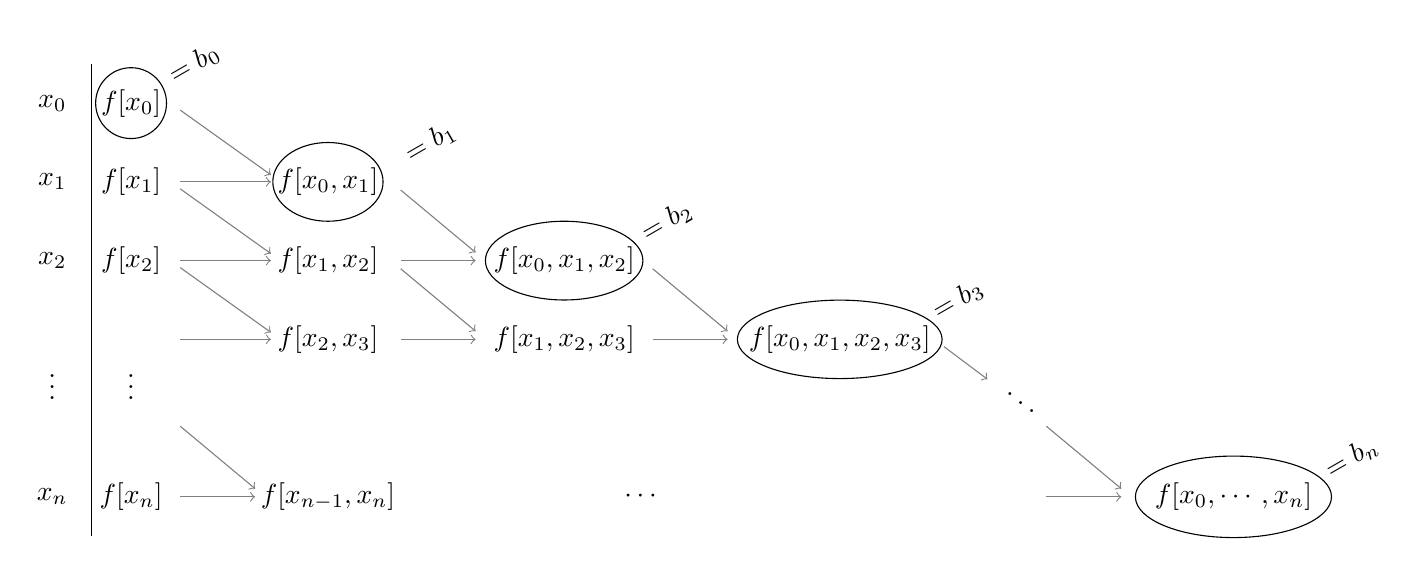
\begin{tikzpicture}

\node at (-0.5, 5.5) {$x_0$};
\node at (-0.5, 4.5) {$x_1$};
\node at (-0.5, 3.5) {$x_2$};
\node at (-0.5, 2) {$\vdots$};
\node at (-0.5, 0.5) {$x_n$};

\draw (0, 6) edge (0,0);

\node (v1) at (0.5,5.5) {$f[x_0]$};
\node at (0.5, 4.5) {$f[x_1]$};
\node at (0.5, 3.5) {$f[x_2]$};
\node at (0.5, 2) {$\vdots$};
\node at (0.5, 0.5) {$f[x_n]$};


\node (v2) at (3,4.5) {$f[x_0, x_1]$};
\node at (3, 3.5) {$f[x_1, x_2]$};
\node at (3, 2.5) {$f[x_2, x_3]$};
\node at (3, 0.5) {$f[x_{n-1}, x_n]$};


\node (v3) at (6,3.5) {$f[x_0, x_1, x_2]$};
\node at (6, 2.5) {$f[x_1, x_2, x_3]$};

\node (v4) at (9.5,2.5) {$f[x_0, x_1, x_2, x_3]$};

\node at (14.5, 0.5) {$f[x_0, \cdots, x_n]$};


\node at (11.8, 1.8) {$\ddots$};

\node (fx0) at (1,5.5) {};
\node (fx1) at (1,4.5) {};
\node (fx2) at (1,3.5) {};
\node (fx3) at (1,2.5) {};
\node (fxn1) at (1,1.5) {};
\node (fxn) at (1,0.5) {};

\node (fx01l) at (2.4,4.5) {};
\node (fx12l) at (2.4,3.5) {};
\node (fx23l) at (2.4,2.5) {};
\node (fxnnl) at (2.2,0.5) {};

\node (fx01r) at (3.8, 4.5) {};
\node (fx12r) at (3.8, 3.5) {};
\node (fx23r) at (3.8, 2.5) {};
\node (fxnnr) at (4, 0.5) {};

\node (fx012l) at (5, 3.5) {};
\node (fx123l) at (5, 2.5) {};

\node (fx012r) at (7, 3.5) {};
\node (fx123r) at (7, 2.5) {};

\node (fx0123l) at (8.2, 2.5) {};
\node (fx0123r) at (10.7, 2.5) {};
\node (fx01234l) at (11.5, 1.9) {};

\node (fx0nl) at (13.2,0.5) {};
\node (fx0n1r) at (12, 0.5) {};
\node (fx0n2r) at (12, 1.5) {};

\draw[gray] [->] (fx0) edge (fx01l);
\draw[gray] [->] (fx1) edge (fx01l);

\draw[gray] [->] (fx1) edge (fx12l);
\draw[gray] [->] (fx2) edge (fx12l);

\draw[gray] [->] (fx2) edge (fx23l);
\draw[gray] [->] (fx3) edge (fx23l);

\draw[gray] [->] (fxn1) edge (fxnnl);
\draw[gray] [->] (fxn) edge (fxnnl);

\draw[gray] [->] (fx01r) edge (fx012l);
\draw[gray] [->] (fx12r) edge (fx012l);

\draw[gray] [->] (fx12r) edge (fx123l);
\draw[gray] [->] (fx23r) edge (fx123l);

\draw[gray] [->] (fx012r) edge (fx0123l);
\draw[gray] [->] (fx123r) edge (fx0123l);

\draw[gray] [->] (fx0123r) edge (fx01234l);

\draw[gray] [->] (fx0n1r) edge (fx0nl);
\draw[gray] [->] (fx0n2r) edge (fx0nl);

\node at (7, 0.5) {$\cdots$};

\draw  (v1) ellipse (0.45 and 0.45);
\draw  (v2) ellipse (0.7 and 0.5);
\draw  (v3) ellipse (1 and 0.5);
\draw  (v4) ellipse (1.3 and 0.4982);
\draw  (14.5,0.5) ellipse (1.2452 and 0.5176);
\node [rotate=30] at (1.3,6) {$=b_0$};
\node [rotate=30] at (4.3,5) {$=b_1$};
\node [rotate=30] at (7.3,4) {$=b_2$};
\node [rotate=30] at (11,3) {$=b_3$};
\node [rotate=30] at (16,1) {$=b_n$};
\end{tikzpicture}

Ten algorytm można wykonywać in situ\footnote{(łac.) w miejscu}.
\end{wniosek}

\begin{proof}

Przez indukcję - wystarczy pokazać, że jeśli jest to prawda dla $k = n-1$, to też dla $k=n$. Niech $p_k$ - wielomian interpolujący Lagrange'a (stopnia $\leq k$) interpolujący $f$ w węzłach $x_0, \cdots, x_k$. Niech $q$ - wielomian interpolacyjny Lagrange'a (stopnia $\leq n-1$) dla węzłów $x_1, \cdots, x_n$. Wtedy:
\[
	p_n(x) = q(x) + \cfrac{x - x_n}{x_n - x_0}(q(x) - p_{n-1}(x))
\]
Rzeczywiście:
\begin{align*}
	p_n(x_n) &= q(x_n) = f(x_n) \\
	p_n(x_i) &= \underbrace{q(x_i)}_{=f(x_i)} + \cfrac{x_i - x_n}{x_n - x_0}(\underbrace{q(x_i)}_{=f(x_i)} - \underbrace{p_{n-1}(x_i)}_{=f(x_i)}) \\
	\vdots & \\
	p_n(x_0) &= q(x_0) + \cfrac{x_0-x_n}{x_n-x_0}(q(x_0) - p_{n-1}(x_0)) = f(x_0)
\end{align*}

\end{proof}

Co można powiedzieć gdy mam reprezentacje takich dwóch wielomianów? W wielomianie $p_n(x)$ (albo $p_1$??) współczynnik przy $x^n$ jest równy $b_n = f[x_0, \cdots, x_n]$. Natomiast współczynnik przy $x^n$ w wielomianie po drugiej stronie $(\star\star): q(x) + \frac{x-x_n}{x_n-x_0}(q(x) - p_n(x))$. Rozpisując $q$ i $p_{n-1}$ w bazie Newtona:
\begin{align*}
	q(x) &= \sum_{i} q(x-x_1)\cdot \cdots \cdot (x-x_i) \\
	p_{n-1}(x) &= \sum_{i} b_i(x-x_1)\cdot \cdots \cdot(x-x_i)
\end{align*}
Wyraz przy najwyższej potędze $x^{n-1}$ to:
\begin{align*}
	q_{n-1} &= f[x_1, \cdots, x_n] \\
	b_{n-1} &= f[x_0, \cdots, x_{n-1}]
\end{align*}
Stąd współczynnik przy $x^n$ w $(\star\star)$ to
\[
\cfrac{1}{x_n-x_0}(f[x_1, \cdots, x_n] - f[x_0, \cdots, x_{n-1}])
\]

Aby wyznaczyć wartość wielomianu interpolacyjnego Lagrange'a w bazie Newtona:
\[
	w(x) = \sum_{i=0}^{n} b_i(x-x_0)\cdot \cdots \cdot (x-x_{i-1})
\]
okazuje się, ze można użyć do tego zmodyfikowanego algorytmu Hornera w koszcie liniowym.

\subsection{Błąd interpolacji}

Gdy mamy do czynienia z funkcją, która jest ``skomplikowana", często dobrze jest zastąpić ją funkcją ``prostszą". Mówimy wtedy o aproksymacji funkcji. Funkcję musimy również aproksymować wtedy, gdy nie jesteśmy w stanie uzyskać pełnej o niej informacji. Na przykład, gdy funkcja reprezentuje pewien proces fizyczny, często zdarza się, że dysponujemy jedynie ciągiem próbek, czyli wartościami tej funkcji w pewnych punktach. Jasne jest, że chcielibyśmy przy tym, aby błąd aproksymacji był możliwie mały.

Podobnie ma się sprawa w przypadku implementacji funkcji elementarnych ($\sin$, $\exp$, ...) w bibliotece funkcji matematycznych, czy wręcz w procesorze. Tam również najchętniej poszukiwalibyśmy sposobu taniego przybliżenia wartości dokładnej funkcji. I rzeczywiście, często w tym celu stosuje się m.in. specjalnie konstruowaną aproksymację wielomianową.

Z tego punktu widzenia, interpolacja wielomianowa może być traktowana jako jeden ze sposobów aproksymacji funkcji, opartym na próbkowaniu. Naturalnym staje się więc pytanie o błąd takiej aproksymacji.

\begin{twierdz}[o najgorszym błędzie interpolacji]
Niech $f \in C^{n+1}[a, b]$\footnote{zbiór funkcji na przedziale $[a, b]$, $(n+1)$-krotnie różniczkowalnych}, $a = x_0 < x_1 < \cdots < x_n = b$ i niech $w_n(x)$ będzie wielomianem interpolacyjnym Lagrange'a dla f na tych węzłach. Wtedy
\[
	\forall_{x \in [a, b]} \exists_{\xi \in (a, b)}\ f(x) - w_n(x) = \cfrac{f^{(n+1)}(\xi)}{(n+1)!}(\omega_n(x))
\]
gdzie $\omega_n(x) = (x-x_0) \cdots (x-x_n)$ (gdzie $\omega(x_i) = f(x_i)$ dla $i = 0, \cdots, n$). (Dowód był)

Przecież $\omega(x_i) = f(x_i)$ dla $i = 0, \cdots, n$ wcale nie zachodzi, bo $\omega(x_i)$ zeruje się dla każdego i, a $f$ niekoniecznie...

\end{twierdz}

\subsection{Interpolacja Hermite'a}

Uogólnieniem rozpatrzonego zadania interpolacji jest zadanie interpolacji Hermite'a\index{interpolacja!Hermite'a}: ``przez zadane węzły $(x_i, y_i)$, $i: 0...n$ poprowadzić wielomian $w$ taki, żeby $w^{(k)}\footnote{\textrm{k-ta pochodna}}(x_i) = y_i^{(k)}$".

\begin{tikzpicture}

\node (v1) at (-0.5,1) {};
\node (v2) at (4,1) {};
\node (v3) at (0,3) {};
\node (v4) at (0,0.5) {};

\draw [->] (v1) edge (v2);
\draw [<-] (v3) edge (v4);

\draw (1, 0.9) edge (1, 1.1);
\draw (2, 0.9) edge (2, 1.1);
\draw (3, 0.9) edge (3, 1.1);

\node at (1, 0.7) {$x_1$};
\node at (2, 0.7) {$x_2$};
\node at (3, 0.7) {$x_3$};

\node[circle,fill,inner sep=1pt] at (1, 2) {};
\node[circle,fill,inner sep=1pt] at (2, 1.4) {};
\node[circle,fill,inner sep=1pt] at (3, 2.3) {};

\node (t1) at (0.5, 2.1) {}; 
\node (d1) at (1.5, 1.9) {}; 

\node (t2) at (1.5, 1.3) {};
\node (d2) at (2.5, 1.5) {};

\node (t3) at (2.5, 2.0) {};
\node (d3) at (3.5, 2.6) {};

\draw (t1) edge (d1);
\draw (t2) edge (d2);
\draw (t3) edge (d3);

\draw [blue] plot[smooth, tension=.5] coordinates {(0.5, 1.5) (1, 2) (2, 1.4) (3, 2.3) (3.5, 2)};
\end{tikzpicture}

Znaleźć wielomian $H_n(x)$ stopnia $\leq n$ taki, że
\[
	H_n^{(j)}(x_i) = f^{(j)}(x_i) \quad i = 0, \cdots, n \quad j = 0, \cdots, n
\] 
\[
	m = (\sum m_i - 1)
\]
To zadanie także ma dokładnie jedno rozwiązanie.

\textbf{Błąd interpolacji:}
\[
f(x) - H_m(x) = \cfrac{f^{n+1}(\xi)}{(m+1)!}w(x)
\]
\[
	w(x) = (x-x_0)^{m_0} \cdot \cdots \cdot (x - x_n)^{m_n}
\]
Dla wyznaczenia wielomianu interpolacyjnego Hermite'a w bazie Newtona (z węzłami krotnymi) działa zmodyfikowany algorytm różnic dzielonych. $m_i$ oznacza krotność $i$-tego węzła, tj. liczba znanych pochodnych + 1. $m_i$ oznacza krotność $i$-tego węzła, tj. liczba znanych pochodnych + 1.

\section{Interpolacja funkcjami sklejanymi (splajny)}
Spójrzmy na interpolację wielomianową w węzłach równoodległych funkcji $f(x) = \cfrac{1}{1+x^2}$

\begin{tikzpicture}

\node (v1) at (-5.5, 0) {};
\node (v2) at (5.5, 0) {};

\draw [->] (v1) edge (v2);
\draw [<-] (0, 5) edge (0, -0.5);

\draw[domain=-2.5:2.5,smooth,scale=2,variable=\x,blue] plot ({\x},{2/(1+\x*\x)});

\draw[red] plot[smooth, tension=.5] coordinates {(0.0, 4.0) (0.58, 3.68) (1.14, 3.1) (1.7, 2.22) (2.28, 1.8) (2.9, 1.14) (3.42, 1.4) (3.8, -1)};

\node at (5, 1.2) {$f(x) = \cfrac{1}{1+x^2}$};

\end{tikzpicture}

Jak widać interpolacja wielomianu wysokiego stopnia w węzłach równoodległych może dawać duży błąd, dlatego potrzebujemy innego sposobu przybliżania skomplikowanych funkcji.

W przeciwieństwie do metody interpolacji Lagrange'a, gdzie stosowaliśmy jeden globalny wielomian dla całego przedziału interpolacji, w metodzie splajnów stosowane są funkcje zdefiniowane jako wielomiany niskiego stopnia osobno dla każdego odcinka pomiędzy sąsiednimi węzłami interpolacyjnymi. Te lokalne wielomiany są jednak tak dobrane, aby - oprócz warunków interpolacji - spełniać warunki sklejenia w taki sposób, aby cały splajn był funkcją o odpowiedniej regularności. Skoncentrujemy się przede wszystkim na zagadnieniu interpolacji za pomocą \texttt{splajnu kubicznego}, tj. funkcji ciągłej wraz z pochodnymi do rzędu drugiego włącznie i zbudowanej z wielomianów 3-ego stopnia. 

\begin{defi}[Splajn] Niech będą dane węzły $a = x_0 < x_1 < \cdots < x_n = b$. Funkcja $s$ jest splajnem stopnia $l$ na $[a, b]$ wtw. \begin{itemize}
\item $s \in C^{l-1}[a, b]$
\item $s|_{[x_i, x_{i+1})}$ - wielomian stopnia $\leq l$
\end{itemize}
\end{defi}

\textbf{Przykład:}

Splajn stopnia 1:
\begin{itemize}
	\item $s \in C^{0}[a, b]$
	\item $s|_{[x_i, x_{i+1})}$ - wielomian stopnia $\leq 1$ (funkcja liniowa)
\end{itemize}

\begin{tikzpicture}

\node (v0) at (-0.5,0) {};
\node (v1) at (7,0) {};
\node (v2) at (0,-0.5) {};
\node (v3) at (0,3) {};

\draw [->] (v0) edge(v1);
\draw [->] (v2) edge(v3);

\draw (2, 0.2) edge (2, -0.2);
\draw (3, 0.2) edge (3, -0.2);
\draw (5, 0.2) edge (5, -0.2);
\draw (6, 0.2) edge (6, -0.2);

\node at (0.3, -0.5) {$x_0$};
\node at (2, -0.5) {$x_1$};
\node at (3, -0.5) {$x_2$};
\node at (5, -0.5) {$x_3$};
\node at (6, -0.5) {$x_4$};

\node [circle,draw=black,fill=white,inner sep=1.5pt] (y1) at (0, 1) {};
\node [circle,draw=black,fill=white,inner sep=1pt] (y2) at (2, 2) {};
\node [circle,draw=black,fill=white,inner sep=1pt] (y3) at (3, 1.7) {};
\node [circle,draw=black,fill=white,inner sep=1pt] (y4) at (5, 2.5) {};
\node [circle,draw=black,fill=white,inner sep=1.5pt] (y5) at (6, 2.3) {};

\draw[blue] (y1) -- (y2) -- (y3) -- (y4) -- (y5);
\end{tikzpicture}

\begin{fakt} Przestrzeń $S_l$ splajnów stopnia $l$ (na ustalonym zestawie węzłów) jest przestrzenią liniową, a jej bazą są funkcje: $\{p_0,p_1, \cdots, p_l, \phi_1, \cdots, \phi_{n-1}\}$, gdzie $p_i(x) = x^i$.
\end{fakt}

\begin{wniosek} Wymiar tej przestrzeni to $n+l$.\end{wniosek}

\textbf{Przykład:}

Funkcja $\phi_i(x) := (x-x_i)^l_+ := \left\{\begin{array}{lr}(x-x_i)^l & dla\ x \geq x_i \\ 0 & x<x_i\end{array}\right.$ też jest splajnem stopnia $l$.

\begin{tikzpicture}

\node (v1) at (-3.5, 0) {};
\node (v2) at (2.5, 0) {};

\draw [->] (v1) edge (v2);
\draw [<-] (-1, 5) edge (-1, -0.5);

\draw[domain=-6:3,smooth,scale=0.5,variable=\x,blue] plot ({\x},{2^(\x)});

\node[rotate=70] at (1.7, 3) {$\phi_i(x)$};

\end{tikzpicture}

W zastosowaniach interpolacyjnych często używamy \texttt{splajnów kubicznych}, czyli $l=3$.

\subsection{Zadanie interpolacji splajnowej} Dla zadanej funkcji $f$, znaleźć splajn $s \in S_l$ taki, że \[s(x_i) = f(x_i)\quad i=0, ..., n\]

Te warunki dają n+1 warunków, a w przypadku interpolacji splajnem ``brakuje" jeszcze dwóch zależności, aby było tyle samo warunków co stopni swobody zadania (bo stopni swobody jest $n+2m-1$).

W ogólności, gdy rozważamy splajny interpolacyjne nieparzystego stopnia, $l=2m-1$ mamy swobodę doboru $2m-2$ dodatkowych warunków. Często są to na przykład:

\begin{itemize}
	\item \textbf{hermitowskie warunki brzegowe}
	Żądam aby nie tylko wartości, ale też ich kolejne pochodne zgadzały się z tym co było powiedziane.
	\[
		s^{(k)}(a) = f^{(k)(a)} \quad k = 1, \cdots, m-1
	\]
	\[
		s^{(k)}(b) = f^{(k)(b)} \quad k = 1, \cdots, m-1
	\]
	
	\item \textbf{naturalne warunki brzegowe}
	\[
		s^{(k)}(a) = s^{(k)}(b) = 0 \quad k = m, \cdots, 2m-2
	\]
	(Jak ktoś wie o co chodziło, proszę o uzupełnienie) Dlaczego naturalne warunki są naturalne? Splajny spełniają pewien specjalny warunek - splajn kubiczny minimalizuje kwadrat z drugiej pochodnej. No - co z tego można by powiedzieć. Dla nas nic, ale dla fizyka od razu coś, bo druga pochodna ma interpretację fizyczną. Krzywizna takiej krzywej jest minimalna pośród tej klasy o której myślimy. Splajn kubiczny jest najgładszy w tej klasie funkcji f. Stąd się bierze naturalny warunek brzegowy. Na krańcach funkcja jest liniowa, a jaka jest druga pochodna funkcji liniowej? Zerowa, stąd te warunki brzego nazywane są naturalnymi.
	
	\item \textbf{periodyczne warunki brzegowe}
	\[
		s^{(k)}(a) = s^{(k)}(b) \quad k=1, \cdots, 2m-2
	\]
\end{itemize}

Dla splajnów kubicznych mamy naturalne warunki brzegowe: $s''(a) = s''(b) = 0$

\subsection{Konstrukcja splajnów}

Zastanówmy się teraz w jaki sposób konstruować splajny.
\subsubsection{Konstrukcja interpolacyjnych splajnów kubicznych}

$s \in C^2[a, b], s|_{[x_i, x_{i+1})}$ - wielomian stopnia $\leq 3$


$s_i := s|_{[x_i, x_{i+1})}$: 

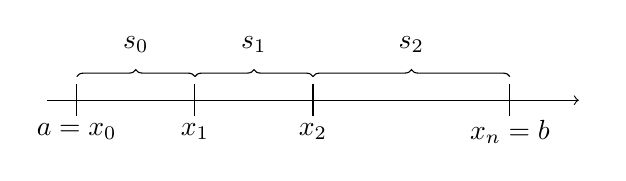
\begin{tikzpicture}
\node (v0) at (0,0) {};
\node (v1) at (7,0) {};

\draw [->] (v0) edge(v1);

\draw (0.5, 0.2) edge (0.5, -0.2);
\draw (2, 0.2) edge (2, -0.2);
\draw (3.5, 0.2) edge (3.5, -0.2);
\draw (6, 0.2) edge (6, -0.2);

\node at (0.5, -0.4) {$a=x_0$};
\node at (2, -0.4) {$x_1$};
\node at (3.5, -0.4) {$x_2$};
\node at (6, -0.4) {$x_n=b$};

\draw[decorate,decoration=brace] (0.5, 0.3) -- node[above=5pt] {$s_0$} (2, 0.3);
\draw[decorate,decoration=brace] (2, 0.3) -- node[above=5pt] {$s_1$} (3.5, 0.3);
\draw[decorate,decoration=brace] (3.5, 0.3) -- node[above=5pt] {$s_2$} (6, 0.3);

\end{tikzpicture}
\[
	s_i(x) = a_i + b_i(x-x_i) + c_i(x-x_i)^2 + d_i(x-x_i)^3
\]

\textbf{Warunki narzucane na splajn}:
\begin{enumerate}
	\item interpolacja: $\underbrace{s_i(x_i)}_{a_i} = f(x_i)$ 
	\item ciagłość II pochodnej:
		\[
			s_i''(x) = 2c_i + 6d_i(x-x_i)
		\]
		\[
			s_i''(x) = s_{i+1}''(x_{i+1})
		\]
		Niech $h = x_{i+1}-x_i$. Jak to sobie rozpiszemy, mamy:
		\begin{align*}
			2c_i + 6d_i \cdot h & = 2c_{i+1} \\
			\implies d_i &= \cfrac{c_{i+1}-c_i}{3h} \quad i=0, ..., n-2
		\end{align*}
		\item ciagłość splajnu w $x_{i+1}$
		\[
			s_i(x_{i+1}) = s_{i+1}(x{i+1})
		\]
		\[
			y_i + b_ih + c_i \cdot h^2 + d_i\cdot h^3 = y_{i+1}
		\]
		Stąd
		\[
			b_i = \cfrac{y_{i+1}-y_i}{h} - \cfrac{h}{3}(c_{i+1} + 2c_i)
		\]
		\item ciągłosć pochodnej w $x_{i+1}$:
		\begin{align*}
			& s_i'(x) = b_i + 2c_i(x-x_i) + 3d_i(x-x_i)^2 \\
			& s_i'(x_{i+1}) = s_{i+1}'(x_{i+1}) \\ 
			(\star) \quad & b_i + 2c_ih + 3d_i\cdot h^2 = b_{i+1}
		\end{align*}
\end{enumerate}

Ponieważ $d_i$ zostało wyliczone w zależności od $\{c_i\}$. Podobnie $b_i$ wyznaczone w zależności od $\{c_i\}$ orz $\{y_i\}$ (ale ten zbiór jest zadany - to po prostu zbiór wartości interpolacji $y_i = f(x_i)$) to podstawiając do $(\star)$ dostajemy zależności wyłącznie pomiędzy $\{c_i\}$ i $\{y_i\}$:
\[
	c_i + 4c_{i+1} + c_{i+2} = \cfrac{3}{h}\left(\cfrac{y_{i+2} - y_{i+1}}{h} - \cfrac{y_{i+1} - y_i}{h}\right) \quad i = 0, \cdots, n-2
\]
To już układ równań liniowych, tyle że ciągle niedookreślony, ponieważ mamy więej niewiadomych niż równań. To są te dwa brakujące wspomniane wcześniej. 

Założenie, że $s''(x_0) = 0 = s''(x_n)$ oznacza, że $c_0 = c_n = 0$.

Macierzowo:
\[
	\left[
		\begin{array}{ccccc}
		4 & 1 & 0 & \cdots & 0 \\ \hline
		1 & \ddots & \ddots & \ddots & \vdots \\
		0 & \ddots & \ddots & \ddots & 0 \\
		\vdots & \ddots & \ddots & \ddots & 1 \\  \hline
		0 & \cdots & 0 & 1 & 4
		\end{array}
	\right]
	\cdot 
	\left[
		\begin{array}{c}
		c_1 \\
		\vdots \\
		\vdots \\
		\vdots \\
		c_{n-1}
		\end{array}
	\right]	
	=
	\left[
		\begin{array}{c}
		g_1 \\
		\vdots \\
		\vdots \\
		\vdots \\
		g_{n-1}
		\end{array}
	\right]	
\]

To macierz symetryczna trójdiagonalna, z dominjącą diagonalą. To jest bardzo dobra wiadomość, bo to oznacza, że ten układ da się rozwiązać kosztem $O(n)$.

\subsection{Błąd interpolacji splajnów} 

\begin{defi}[przypomnienie z analizy]
	$\norm{f}_\infty = sup_{x \in [a, b]}|f(x)|$
\end{defi}

\begin{twierdz}[o aproksymacji naturalnym splajnem kubicznym interpolującym f] Niech $f \in C^2[a, b]$. Niech $a = x_0 < x_1 < \cdots < x_n = b$ będą węzłami równoodległymi, $x_{i+1} - x_i = h$ (dla $i=0, ..., n)$. Wtedy
\[
	\norm{f-s}_\infty \leq C \cdot \norm{f''}_\infty \cdot h^2 = O(h^2)
\]
\end{twierdz}

\textbf{Dowód:}

Niech $x \in [x_i, x_{i+1})$. Podstawiając to co wiemy o $s_i$ ($s_i(x) = s|_{[x_i, x_{i+1})}$) do wzoru na $s_i(x)$:
\begin{align*}
	s_i(x) & = a_i + b_i(x-x_i) + c_i(x-x_i)^2 + d_i(x-x_i)^3 \\
	& = f(x_i) + \cfrac{f(x_{i+1}) - f(x_i)}{h}(x-x_i) + \left( c_i(x-x_i)^2 - \cfrac{h}{3}(c_{i+1}) + 2c_i) \cdot (x-x_i) + \cfrac{c_{i+1} - c_i}{3h}(x-x_i)^3 \right)
\end{align*}
Zauważmy, że wyrażenie w nawiasie szacuje się przez:
\[
	\underbrace{C}_{\textrm{pewna stała}} \cdot \max\limits_{i}|c_i| \cdot h^2
\]
Zatem
\begin{align*}
	|s_i(x) = f(x)| & = |f(x_i) + \cfrac{f(x_{i+1}) - f(x_i)}{h}(x-x_i) + \left( \begin{array}{c}\\ \cdots \end{array} \right) - f(x)| \\
	& \leq |f(x_i) - f(x) + \cfrac{f(x_{i+1}) - f(x_i)}{h}(x-x_i) + C \cdot \max\limits_{i}|c_i| \cdot h^2| \\
	& \leq |\underbrace{f'(\xi) \cdot (x_i - x) - f'(\nu)\cdot(x_i-x)}_{(\underbrace{f'(\xi) - f'(\nu)}_{f''(\kappa) \cdot(\xi - \nu)})\cdot(x_i-x)}| + C \cdot \max\limits_i|c_i|\cdot h^2 \\
	& \leq \underbrace{|f''(\kappa)|}_{\norm{f''}} \cdot h^2 + C \cdot \max\limits_i |c_i| \cdot h^2
\end{align*}
Wystarczy więc wykazać, że $\max\limits_i |c_i| \leq const\cdot \norm{f''}$. $c = [c_1, \cdots, c_{n-1}]^T$ spełnia układ równań:
\[
	A \cdot c = g
\]
gdzie $g_i = \cfrac{3}{h} \cdot \left(\underbrace{\underbrace{\cfrac{f(x{i+1}) - f(x_i)}{h}}_{f'(\hat{\xi})} - \underbrace{\cfrac{f(x_i) - f(x_{i-1})}{h}}
_{f'(\hat{\nu})}}_{f''(\hat{\kappa}(\hat{\xi} - \hat{\nu})} \right)$

Zatem $|g_i| \leq \cfrac{3}{h} \cdot |f''(\hat{\xi_i})| \cdot |\underbrace{\hat{\xi_i} - \hat{\nu_i}}_{\leq h}| \leq 3 \cdot |f''(\hat{\kappa_i})| \leq 3 \cdot \norm{f''}$. Ale
\[
	c = A^{-1}\cdot g
\]
więc
\[
	\max\limits_i|c_i| = \norm{c}_\infty = \norm{A^{-1}g}_\infty \leq \norm{A^{-1}}_\infty \cdot \norm{g}_\infty
\]

\[
	A = \left[
		\begin{array}{ccc}
		4 & 1 & \\
		1 & \ddots & \ddots \\
		& \ddots & 4
		\end{array}
	\right]
	 = 4 \cdot  \left[
		\begin{array}{ccc}
		1 & \frac{1}{4} & \\
		\frac{1}{4} & \ddots & \ddots \\
		& \ddots & 1
		\end{array}
	\right]
	= 4(I + \underbrace{\left[
		\begin{array}{ccc}
		0 & \frac{1}{4} & \\
		\frac{1}{4} & \ddots & \ddots \\
		& \ddots & 0
		\end{array}
	\right]}_{M})
\]
\[
	A^{-1} = \cfrac{1}{4} (I + M)^{-1}
\]
$(I + M)$ jest nieosobliwe o ile $\norm{M} < 1$. Ponadto $\norm{(I+M)^{-1}}_\infty \leq \cfrac{1}{1-\norm{M}_\infty}$
\[
	\norm{A^{-1}}_\infty = \cfrac{1}{4} \cdot \norm{(I+M)^{-1}}_\infty \leq \cfrac{1}{4} \cdot \cfrac{1}{1-\norm{M}_\infty} = \cfrac{1}{2}
\]

\begin{twierdz}[o błędzie aproksymacji interpolacja splajnem kubicznym z Hermitowskimi warunkami brzegowymi]
	Niech $s \in S_3[a, b]$ będzie splajnem interpolacyjnym kubicznym z Hermitowskimi warunkami brzegowymi, tzn: \[s(x_i) = f(x_i) \quad i=0, ..., n\] oraz \[s'(a) = f'(a) \quad s'(b) = f'(b)\] przy czym dla urposzczenia węzły są równoodległe ($h = x_{i+1}-x_i$). Wtedy jeśli $f \in C^4[a, b]$, to: 
	\[ 
		\norm{f-s}_\infty \leq \cfrac{5}{384} \cdot h^4 \cdot \norm{f^{(4)}}_\infty
	\]
	\[ 
		\norm{f'-s'}_\infty \leq \cfrac{1}{24} \cdot h^3 \cdot \norm{f^{(4)}}_\infty
	\]
	\[ 
		\norm{f''-s''}_\infty \leq \cfrac{3}{8} \cdot h^2 \cdot \norm{f^{(4)}}_\infty
	\]
\end{twierdz}

\subsection{Krzywe B-splajne (B-spline)}

Krzywa B-sklejana jest jedną z najczęściej stosowanych reprezentacji parametrycznych krzywych sklejanych. Angielska nazwa spline wzięła się z gwary kreślarzy i odnosiła do długiej elastycznej metalowej taśmy, której używano do rysowania samolotów, samochodów, statków itp. Zawieszając odpowiednio dobrane obciążniki można było uzyskać krzywą o ciągłości geometrycznej drugiego rodzaju. Angielska nazwa krzywych B-sklejanych – B-spline jest skrótem od basis spline function, co znaczy "funkcja bazowa splajnów". Chociaż biorąc pod uwagę wykres, który wygląda jak dzwon, można też uznać, że pochodzi to od słowa ``bell" :-).

\begin{defi}[nośnik funkcji]
Niech $f: \RR \ra \RR$, określamy nośnik funkcji jako:
\[
	supp(f) = \{x \in \RR: f(x) \neq 0\}
\] 
\end{defi}

\textbf{Przykład}

$S_0$ - funkcje kawałkami stałe:

\begin{tikzpicture}	
	\draw (-3, -1) -- (10, -1);
	
	\foreach \x in {-2, -1, 0, 1, 2, 3, 4, 5, 8, 9}
	\draw (\x,-0.8) -- (\x,-1.2);
	\foreach \x in {-2, -1, 0, 1, 2, 3, 4, 5}
	\node at (\x, -1.5) {$x_{\x}$};
	
	
	\node at (8, -1.5) {$x_{n}$};
	\node at (9, -1.5) {$x_{n+1}$};
	
	\draw (0, 0) -- (1, 0);
	\draw (1, -2) -- (2, -2);
	\draw (2, 0.5) -- (8, 0.5);
	
	\node [circle,draw=black,fill=white,inner sep=1.5pt] at (0, 0) {};
	\node [circle,draw=black,fill=none,inner sep=1.5pt] at (1, 0) {};
	\node [circle,draw=black,fill=white,inner sep=1.5pt] at (1, -2) {};
	\node [circle,draw=black,fill=none,inner sep=1.5pt] at (2, -2) {};
	\node [circle,draw=black,fill=white,inner sep=1.5pt] at (2, 0.5) {};
	\node [circle,draw=black,fill=none,inner sep=1.5pt] at (8, 0.5) {};
\end{tikzpicture}

W tej przestrzeni mogę zdefiniować bazę $B_i^0(x)$:

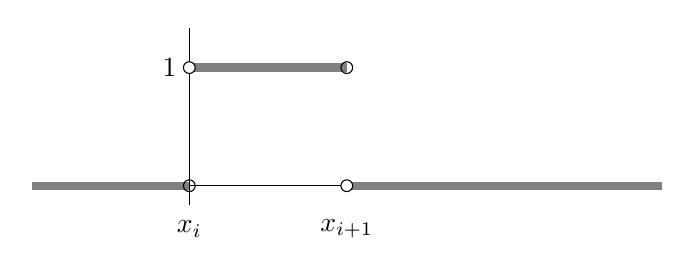
\begin{tikzpicture}
\draw (0,0) -- (8, 0);
\draw (2, 2) --(2, -0.25);
\draw[line width=3,gray] (0, 0) -- (2, 0);
\draw[line width=3,gray] (2, 1.5) -- (4, 1.5);
\draw[line width=3,gray] (4,0) -- (8, 0);

\node at (2, -0.55) {$x_i$};
\node at (4, -0.55) {$x_{i+1}$};

\node [circle,draw=black,fill=white,inner sep=1.5pt] at (2, 1.5) {};
\node [circle,draw=black,fill=none,inner sep=1.5pt] at (4, 1.5) {};

\node [circle,draw=black,fill=white,inner sep=1.5pt] at (4, 0) {};
\node [circle,draw=black,fill=none,inner sep=1.5pt] at (2, 0) {};

\node at (1.75, 1.5) {$1$};
\end{tikzpicture}

Zauważmy, że $S_0 = span\left\{B_i^0\right\}_{i=0}^{n-1}$.
\[
	supp(B_i^0(x)) = [x_i, x_{i+1}) \quad \la \textrm{nośnik funkcji}
\]
\[
	B_i^0(x) \geq 0
\]
\[
	\sum_{i=-\infty}^{\infty} B_i^0(x) = 1
\]

Suma wygląda na nieskończoną, ale tylko pozornie. Bowiem gdy ustalę wartość $x$, to ten $x$ wpada do konkretnego jednego przedziału i wtedy w tej sumie tylko jednen składnik jest niezerowy.

\textbf{Przykład} $S_1$ - funkcje ciągłe, kawałkami liniowe:

\begin{tikzpicture}	
	\draw (-3, -1) -- (8, -1);
	
	\foreach \x in {-2, -1, 0, 1, 2, 6, 7}
	\draw (\x,-0.8) -- (\x,-1.2);
	\foreach \x in {-2, -1, 0, 1, 2}
	\node at (\x, -1.5) {$x_{\x}$};
	
	\node at (6, -1.5) {$x_{n}$};
	\node at (7, -1.5) {$x_{n+1}$};
	
	\draw (-2, 0.5) -- (-1, 1);
	\draw (-1, 1) -- (0, 0.6);
	\draw (0, 0.6) -- (1, 1.1);
	\draw (1, 1.1) -- (2, 0.5);
	\draw (2, 0.5) -- (3, 0.5);
	\draw[dashed] (3, 0.5) -- (4, 0.5);
	\draw (4, 0.5) -- (5, 0.5);
	\draw (5, 0.5) -- (6, 1);
	\draw (6, 1) -- (7, 0.5);
\end{tikzpicture}

Baza dla tej przestrzeni funkcji:

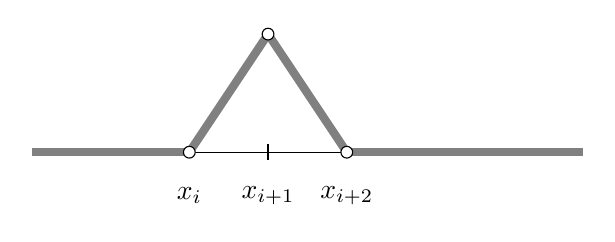
\begin{tikzpicture}
	\draw (0,0) -- (7, 0);
	\draw[line width=3,gray] (0, 0) -- (2, 0);
	\draw[line width=3,gray] (2, 0) -- (3, 1.5);
	\draw[line width=3,gray] (3, 1.5) -- (4, 0);
	\draw[line width=3,gray] (4,0) -- (7, 0);

	\draw (3, 0.1) -- (3, -0.1);

	\node at (2, -0.55) {$x_i$};
	\node at (3, -0.55) {$x_{i+1}$};
	\node at (4, -0.55) {$x_{i+2}$};

	\node [circle,draw=black,fill=white,inner sep=1.5pt] at (2, 0) {};
	\node [circle,draw=black,fill=white,inner sep=1.5pt] at (3, 1.5) {};
	\node [circle,draw=black,fill=white,inner sep=1.5pt] at (4, 0) {};
\end{tikzpicture}

Co więcej ta baza ma podobne właśniwości jak ta z poprzedniego przykładu! 
\[
	supp(B_i^1(x)) = (x_i, x_{i+2})
\]
\[
	B_i^1(x) \geq 0
\]
\[
	\sum_{i=-\infty}^{\infty} B_i^1(x) = 1
\]

Będziemy chcieli konstruować takie bazy, ktorych nośnik funkcji jest możliwie mały. Tak więc nasz cel: skontruować bazę przestrzeni splajnów $S_k$ składającą się z funkcji o ``małym" nośniku. Np. dla $S_3$ (przestrzeni splajnów kubicznych).

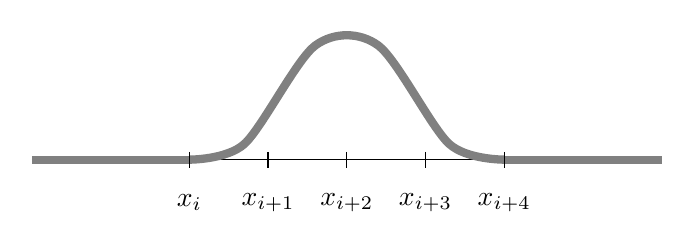
\begin{tikzpicture}
	\draw (0,0) -- (8, 0);
	%\draw[line width=3,gray] (0, 0) -- (2, 0);
	
	\draw[line width=3,gray] (0, 0) -- (2, 0);
	\draw[line width=3,gray] (6, 0) -- (8, 0);
	\draw[line width=3,gray] plot[smooth, tension=.5] coordinates {(2, 0) (2.7, 0.2) (3.6, 1.45) (4.4, 1.45) (5.3,0.2) (6, 0)};

	\foreach \x in {2, 3, 4, 5, 6}
		\draw (\x, 0.1) -- (\x, -0.1);

	\node at (2, -0.55) {$x_i$};
	\node at (3, -0.55) {$x_{i+1}$};
	\node at (4, -0.55) {$x_{i+2}$};
	\node at (5, -0.55) {$x_{i+3}$};
	\node at (6, -0.55) {$x_{i+4}$};

\end{tikzpicture}


\begin{defi}
Niech:
\[
	B_i^k(x) := V_i^k(x) \cdot B_i^{k-1}(x) + (1-V_{i+1}^k(x)) \cdot B_{i+1}^{k-1}(x)
\]
gdzie
\[
	V_i^k(x) := \cfrac{x-x_i}{x_{i+k} - x_i}
\]
Zauważmy, że $B_i^k(x)$ jest na każdym przedziale $[x_i, x_{i+1})$ wielomianem stopnia $\leq k$.
\end{defi}

\subsubsection{Własności B-splajnów}
\begin{itemize}
	\item \textbf{Ograniczony nośnik:}
	
	Jeśli $x \not\in (x_i, x_{i+k+1}$, to $B_i^k(x) = 0$.
	
	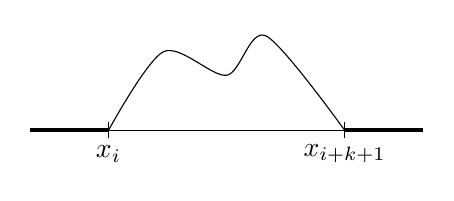
\begin{tikzpicture}
		\draw (0,0) -- (5, 0);
		\draw[line width=1.5] (0,0) -- (1, 0);
		\draw[line width=1.5] (4,0) -- (5, 0);

		\draw plot[smooth, tension=.5] coordinates {(1,0) (1.7, 1) (2.5, 0.7) (3, 1.2) (4, 0)};

		\draw (1, -0.1) -- (1, 0.1);
		\draw (4, -0.1) -- (4, 0.1);
		\node at (1, -0.3) {$x_i$};
		\node at (4, -0.3) {$x_{i+k+1}$};
	\end{tikzpicture}
	
	\begin{proof}
	$k = 1 \implies$ prawda
	
	Załóżmy, że $k-1$ - prawdziwe, czy $k$ też prawda?
	
	Skoro tak, to $B_i^{k-1} = 0$ dla $x \not\in (x_i, x_{i+(k-1)+1}) = (x_i, x_{i+k})$.
	
	$B_{i+1}^{k-1}(x) = $ dla $x \not\in (x_{i+1}, x_{i+k+1})$.
	
	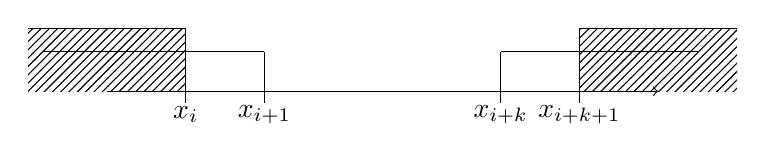
\begin{tikzpicture}
		\draw [->] (0,0) -- (7, 0);
		
		\fill [pattern=north east lines, pattern color=black] (-1,0.8) rectangle (1,0);
		\draw (-1,0.8) -- (1, 0.8);
		\draw (1, 0.8) -- (1,-0.15);
		
		\draw (-0.8, 0.5) -- (2, 0.5);
		\draw (2, 0.5) -- (2, -0.15);
		
		\fill [pattern=north east lines, pattern color=black] (8,0.8) rectangle (6,0);
		\draw (8,0.8) -- (6, 0.8);
		\draw (6, 0.8) -- (6,-0.15);
		
		\draw (5, 0.5) -- (7.5, 0.5);
		\draw (5, 0.5) -- (5, -0.15);
		
		\node at (1, -0.3) {$x_i$};
		\node at (2, -0.3) {$x_{i+1}$};
		\node at (5, -0.3) {$x_{i+k}$};
		\node at (6, -0.3) {$x_{i+k+1}$};
	\end{tikzpicture}
	
	Więc ich kombinacja liniowa równa się $0$ dla $x \not\in (x_i, x_{i+k+1})$.
	\end{proof}
	
	\item Obliczanie wartości $\sum_{i=-\infty}^{\infty} c_i \cdot B_i^k(x)$ dla wskazanego $x$. Zwróćmy uwagę, że znów dzięki temu że funkcje bazowe mają ograniczony nośnik to dla ustalonego $x$ jest tylko skończona liczba funkcji, gdzie składnik sumy jest niezerowa. Dlatego nieskońćzona suma zredukuje się do skończonej sumy, bo pozostałe składniki są mnożone przez $0$.
	
	Zauważmy, że:
	\[
		\sum_{i=-\infty}^{\infty} c_i^k B_i^k(x) = \sum_{i=-\infty}^{\infty}(\underbrace{c_i^k V_i^k(x) + c_{i-1}^k(1-V_i^k(x))}_{c_i^{k-1}}) \cdot B_i^{k-1}(x)
	\]
%	Rzeczywiście:
%	\[
%		\sum c_i B_i^k(x) = \sum c_i(V_i^k \cdot )
%	\]
\end{itemize}

\begin{wniosek}[Algorytm (de Boor'a) obliczania wartości s(x)]
	\[
		s(x) = \sum_{i=-\infty}^{+\infty} c_i^kB_i^k(x)
	\]
	Niech $c_i^{k-1} = c_i^k \cdot V_i^k(x) + c_{i-1}^k(1- V_i^k)$. Zatem
	\[
		S(x) = \sum c_i^k\cdot B_i^k(x) = \sum c_i^{k-1} \cdot B_i^{k-1}(x) = \cdots = \sum c_i^0 B_i^0(x)
	\]
	A $B_i^0$ już znamy. Jeśli więc $x \in [x_m, x_{m+1})$, to $\sum c_i^0 B_i^0(x) = c_m^0$. Algorytm:
	
	\begin{tikzpicture}
		\node[anchor=west] at (0, 4) {$c_{m}^{k}$};
		\node[anchor=west] at (0, 3) {$c_{m-1}^{k}$};
		\node[anchor=west] at (0, 2) {$c_{m-2}^{k}$};
		\node[anchor=west] at (0, 1) {$\ \ \vdots$};
		\node[anchor=west] at (0, 0) {$c_{m-k}^{k}$};
		
		\node[anchor=west] at (2.5, 4) {$c_{m}^{k-1}$};
		\node[anchor=west] at (2.5, 3) {$c_{m-1}^{k-1}$};
		\node[anchor=west] at (2.5, 1) {$c_{m-k+1}^{k-1}$};
		
		
		\node at (9, 4) {$c_{m}^{1}$};
		\node at (9, 3) {$c_{m-1}^{1}$};
		\node at (12, 4) {$c_{m}^{0}=s(x)$};
		
		\node (cmkr) at (1, 4) {};
		\node (cm1kr) at (1, 3) {};
		\node (cm2kr) at (1, 2) {};
		\node (cm3kr) at (1, 1) {};
		\node (cmkkr) at (1, 0) {};
		
		\node (cmk1l) at (2.6, 4) {};
		\node (cm1k1l) at (2.6, 3) {};
		\node (cm3k1l) at (2.6, 1) {};
		
		\node (cmk1r) at (3.7, 4) {};
		\node (cm1k1r) at (3.7, 3) {};
		\node (cm3k1r) at (3.7, 1) {};
		
		\node (cm1l) at (8.5, 4) {};
		\node (cm11l) at (8.5, 3) {};
		
		\node (cm1r) at (9.5, 4) {};
		\node (cm11r) at (9.5, 3) {};
		\node (cm0l) at (11.2, 4) {};
		
		\draw [->] (cmkr) -- (cmk1l);
		\draw [->] (cm1kr) -- (cmk1l);
		\draw [->] (cm1kr) -- (cm1k1l);
		\draw [->] (cm2kr) -- (cm1k1l);
		\draw [->] (cm3kr) -- (cm3k1l);
		\draw [->] (cmkkr) -- (cm3k1l);
		
		\draw [->] (cmk1r) -- (5, 4);
		\draw [->] (cm1k1r) -- (5, 3.9);
		\draw [->] (cm1k1r) -- (5, 3);
		\draw [->] (cm3k1r) -- (5, 1.55);
		
		\draw [->] (cm1r) -- (cm0l);
		\draw [->] (cm11r) -- (cm0l);
		
		\draw [->] (7, 4) -- (cm1l);
		\draw [->] (7, 3.05) -- (cm1l);
		\draw [->] (7, 3) -- (cm11l);
		\draw [->] (7, 2.4) -- (cm11l);
		
		\draw [dashed] (5.3, 4) -- (6.7, 4);
		\draw [dashed] (5.3, 3) -- (6.7, 3);
		\draw [dashed] (5.3, 1.69) -- (6.7, 2.26);
		
	\end{tikzpicture}
\end{wniosek}

\subsubsection{Unormowanie B-splajnów}
Unormowanie B-splajnów: 
\[
	\sum_{i=-\infty}^{\infty} B_i^k(x) \equiv 1
\]

\begin{proof}
\[
\sum 1 \cdot B_i^k(x) = \sum \underbrace{(1 \cdot V_i^k(x) + 1 \cdot (1-V_i^k(x))}_{=1} \cdot B_i^{k-1}(x) = \sum B_i^{k-1}(x)
\]
Dowód przez indukcję.
\end{proof}

\begin{fakt}[Pochodna B-splajnu]
	\[
		\cfrac{d}{dx} B_i^k(x) = k \cdot (\alpha_i^k \cdot B_i^{k-1}(x) - \alpha_{i+1}^k \cdot B_{i+1}^{k-1}(x))
	\]
	gdzie
	\[
		\alpha_i^k := \cfrac{d}{dx}V_i^k(x) = \cfrac{1}{x_{i+k} - x_i}
	\]
\end{fakt}
\begin{wniosek}
	\[
		\cfrac{d}{dx}(\sum_{i=-\infty}^{\infty} c_i B_i^k(x)) = k \cdot \sum_{i=-\infty}^{\infty} \cfrac{c_i - c_{i-1}}{x_{i+k}-x_i} \cdot B_i^{k-1}(x)
	\]
	co można też obliczyć algorytmem de Boor'a
\end{wniosek}
\begin{wniosek}
	Dla $k \geq 1$, $B_i^k \in C^{k-1}(\RR)$ (czyli B-splajny rzeczywiście są splajnami)
\end{wniosek}

\begin{twierdz}
	Funkcje $\{B_{-k}^k, B_{-k+1}^k, \cdots, B_{n-1}^{k}\}$ tworzą bazę splajnów $S_k$ na przedziale $[a, b]$ ($a = x_0 < x_1 < \cdots < x_n = b$)
\end{twierdz}
\begin{wniosek}
	Jeśli $s \in S_k$, to istnieją $\{c_i\}$ takie, że:
	\[
		s(x) \equiv \sum_{i=-k}^{n-1} c_i \cdot B_i^k(x)
	\]
\end{wniosek}

\section{Aproksymacja funkcji}
Dziś postaramy odpowiedzieć na pytanie: ``jak najlepiej aproksymować funkcje"?

\textbf{Zadanie najlepszej aproksymacji}

$f \in F \la \textrm{przestrzeń unormowana (bo musimy jakoś liczyć ten błąd}$

Szukamy $v^\star \in V \subset F$, który najlepiej przybliża $f$ wśród wszystkich elementów z $V$.

Najlepiej przybliża, tzn. błąd aproksymacji $f$ przez $v$ będzie najlepszy możliwy: $\norm{f-v^\star} \leq \norm{f-v} \quad \forall_{v \in V}$. Wtedy $v^\star$ to element najlepszej aproksymacji (ENA). Nie wiemy czy taki element istnieje ani czy jest jeden lub więcej.

\begin{fakt} Jeśli $F$ - przestrzeń liniowa, $V \subset F$ jest jej podprzestrzenią liniową skończonego wymiaru, to dla każdego $f \in F$ istnieje ENA $v^\star \in V$.\end{fakt}

\textbf{Przykład:}

$F = C^0(a, b) \la \textrm{klasa funkcji ciągłych w [a, b]}$

Jest to oczywiście przestrzeń liniowa. Zatem mówimy o ``aproksymacji funkcji ciągłej na [a, b]". Jakie wybrać $V$? Mamy dużo możliwości:
\[
	V := \left\{ \begin{array}{ll}
		\mathbb{P}_n & \textrm{przestrzeń liniowa wielom. stopnia} \leq n \\
		S^l & \textrm{przestrzeń liniowa splajnów stopnia} \leq l\textrm{ opartych na węzłach }x_1, ..., x_n\\
		\{\sum_{i=0}^{n} \alpha_i e^{-\beta_j * t} : \alpha_i \in \RR\} & gdzie\ 0 \leq \beta_0 < ... < \beta_n \\
		gdy\ [a, b] = [0, 2\pi] & V = span\{1, \sin{t}, \cos{t}, \sin{2t}, \cos{2t}, \cdots, \sin{nt}, \cos{nt} \} \quad \textrm{przestrzeń wielomianów trygonometrycznych}
   \end{array}\right.
\]

Po co w ogóle to robić? Bo $F$ to przestrzeń nieskończonego wymiaru, a wszystkie przedstawione podprzestrzenie $V$ są skończonego wymiaru i można je łatwiej określać, prościej liczyć, wygodnie przechowywać w komputerze i mają wiele innych zalet.

Musimy zdecydowań się na jakąś normę i znowu mamy tutaj wiele możliwości, np.

\[
	\begin{array}{l|l}
		nazwa & wzor \\ \hline
		L^1(a, b) & \norm{f}_1 := \int_a^b |f(t)| dt \\
		L^2(a, b) & \norm{f}_2 := \sqrt{\int_a^b |f(t)|^2 dt} \textrm{(aproksymacja średniokwadratowa)} \\
		C^0(a, b) & \norm{f}_\infty := \max_{t \in [a, b]} |f(t)| \textrm{(aproksymacja jednostajna)}\\
		L^2_\rho(a, b) & \norm{f}_{2, \rho} := \sqrt{\int_a^b |f(t)|^2 \rho(t) dt} \quad \rho(t) > 0\ na\ [a, b] \\ \hline
		\multicolumn{2}{l}{\textrm{ustalone punkty }t_0, \cdots, t_N} \\ \hline
		l_1\ dyskretna & \sum_{i=0}^N |f(t_i)| \\
		l_2\ dyskretna & \sqrt{\sum_{i=0}^N |f(t_i)|^2} \\
		l_\infty\ dyskretna & \max_{i} |f(t_i)| \\
		l_{2,\rho}\ dyskretna ?? & \sqrt{\sum_{i=0}^N \rho(t_i) |f(t_i)|^2} ???
	\end{array}
\]

Te wzory oczywiście różnią się od siebie:

\begin{tikzpicture}

\end{tikzpicture}

$v_1$ ``dobrze" aproksymuje funkcję $f$ w normie $L^2$ (bo mam całkować kwadrat różnicy. I mimo dużej różnicy na małym przedziale, to ze względu na małą miarę tego przedziału i tak norma daje przyzwoity wynik). Ale jednocześniej $v_1$ źle aproksymuje $f$ w normie supremum, bo na tym małym przedziale różnica jest ogromna. Mało tego! Ta funkcja $v_1$ lepiej aproksymuje w normie $L^2$ niż funkcja $v_2$, ale jednocześniej $v_2$ lepiej aproksymuje $f$ niż $v_1$ w normie supremum!

\textrm{Aproksymacja w przestrzeni unitarnej}

Niech $H$ - przestrzeń liniowa z iloczynem skalarnym $(x, y)$ dla $x, y \in H$ (np. $H:=\RR^n \quad (x, y) := x^Ty = \sum_i^n x_i, y_i$)

(np. $H:=C^0[a, b] \quad (f, g) := \int_a^b f(t)g(t) dt$)

Ten iloczyn skalarny indukuje w $H$ normę:
\[
	\norm{f} = \sqrt{(f, f)}
\]

\begin{twierdz}[o charakteryzacji ENA w przestrzeni unitarnej]
Niech $V \subset H$ będzie podprzestrzenią liniową w $H$. $v^\star \in V$ jest ENA dla $f \in H \iff (f-v^\star, v) = 0 \ \forall_{v \in V}$ 
\end{twierdz}

(mini ryunek przestrzeni i prostopadłego wektora)

\begin{proof}
``$\impliedby$"

Dla dowolnego $v \in V$:
\[
	\begin{array}{rl}
	\norm{f-v}^2 & = \norm{f - v^\star + \underbrace{v^\star - v}_{w \in V}}_2^2 \\
	& = (f-v^\star + w, f-v^\star + w) \\
	& = (f-v^\star, f-v^\star) + (w, f-v^\star) + (f-v^\star, w) + (w, w) \\
	& = \norm{f-v^\star}^2 + \underbrace{\norm{w}^2}_{\geq 0} + 2\underbrace{(w, f-v^\star)}_{=0} \\
	& \geq \norm{f-v^\star}^2
	\end{array}
\]

``$\implies$"

Weźmy $h \in V$ oraz $\lambda > 0$.
\[
	\begin{array}{rl}
	\norm{f-v^\star}^2 & \leq \norm{f-v^\star + \lambda*h}^2 \\
		& = \norm{f-v^\star}^2 + \lambda^2\norm{h}^2 + 2\lambda(f-v^\star, h)
	\end{array}
\]
Stąd:
\[
	0 \leq \lambda * \norm{h}^2 + 2(f-v^\star, h)
\]
Biorąc $\lambda \searrow 0$ dostajemy $0 \leq 2(f-v^\star, h)$

Biorąc zamiast $h$ wektor $-h$ dostajemy: $0 \leq \lambda \norm{h}^2 - 2(f - v^\star, h)$

$\lambda \searrow 0 \implies$
\[
	0 \leq -2(f-v^\star, h)
\] 
czyli
\[
 	(f - v^\star, h) \leq 0
\]
Skąd
\[
	(f-v^\star, h) = 0 \quad \forall_{h \in V}
\]

\end{proof}

Bycie optymalnym oznacza, że wektor błędu jest prostopadły do tej przestrzeni. To wygląda jak ciekawostka teoretyczna, ale to prowadzi do algorytmu!

\begin{wniosek}
	Jeżeli $V$ jest skończonego wymiaru to ENA istnieje i jest jedyny. Gdy $\{v_i\}^n_{i=0}$ są bazą przestrzeni $V$, to $v^\star = \sum_{i=1}^n \alpha_i^\star v_i$ i współczynniki $\{\alpha_i^\star\}$ istnieją?
\end{wniosek}

\[
	\left[
		\begin{array}{ccc}
		(v_1,v_1) & \cdots & (v_1, v_n) \\
		\vdots & (v_i, v_j) & \vdots \\
		(v_, v_i) & \cdots & (v_n, v_n)
		\end{array}
	\right]
	\cdot
	\left[
		\begin{array}{c}
		\alpha_1^\star \\ \vdots \\ \alpha_n^\star
		\end{array}
	\right]
	=
	\left[
		\begin{array}{c}
		(f, v_1) \\
		\vdots \\
		(f, v_n)
		\end{array}
	\right]
\]
(układ równań normalnych)

Dowód:
\[
	(f- v^\star, v) = 0 \quad \forall_{v \in V}
\]
Zatem także dla $v = v_j$:
\[
	(f-v^\star, v_j) = 0 \quad \forall_{j = 1, \cdots, n}
\]
\[
	\underbrace{(\sum \alpha_i^\star *v_i, v_j)]}_{\sum \alpha_i^\star(v_i, v_j)} = (v^\star, v_j) = (f, v_j) \quad \textrm{Układ h równań z n niewiadomymi}
\]

Macierz $\left[ \begin{array}{c} (v_i, v_j) \end{array} \right]_{i, j=1}^n$ jest
\begin{itemize}
	\item symetryczna
	\item dodatnio określona (jako macierz Gramma)
\end{itemize}

Układ ma więc dokładnie 1 rozwiązanie.

\textbf{Uwaga} Macierz Gramma jest zazwyczaj gęsta i w wielu przypadkach źle uwarunkowana. Jest SPD (symetryczna i dodatnio określona)), więc zadziała algorytm Choleskiego (koszt $O(n^3)$).

Możemy uprościć zadanie wyznaczania ENA przez odpowowiedni dobór bazy:

Wybierając bazę orogonalną w $V$:
\[
	V = span\{p_i, p_j\} = 0 \quad dla\ i \neq j
\]
Dostajemy macierz Gramma (diagonalną)
\[
	\left[
		\begin{array}{ccc}
		(p_1,p_1) &  &  \\
		 & \ddots & \\
		 &  & (p_n, p_n)
		\end{array}
	\right]
\]
i w konsekwencji:
\[
	v^\star = \sum_{i=1}^n \cfrac{(f, p_i)}{(p_i, p_i)}p_i
\]
Gdyby dodatkowo $\{p_i\}$ były unormowane, $\norm{p_i} = 1$ to wtedy ENA jest dana:
\[
	v^\star = \sum_{i=1}^{n}(f, p_i) \cdot p_i
\]

Tylko czy łatwo wybrać bazę ortogonalną w przestrzeni wielomianów?

\subsection{Wielomiany ortogonalne}

Zrobimy to dla przypadku iloczynu skalarnego w $L^2_\rho(a, b)$: $(f, g) = \int_a^b f(x)g(x)\rho(x)dx$

$\rho$ - funkcja wagowa $\rho > 0$ na $[a, b]$, $\norm{f}_{2, \rho} = \sqrt{(f, f)}$

\begin{twierdz}[formuła trójczłonowa]
	Wielomiany $\{P_k\}$, $k = 0, 1, ...$ postaci
	\[
		P_k = x^k + ...\textrm{(niższe potęgi)}...
	\]
	wyrażają się wzorem:
	\[
		P_k(x) = (x + \beta_k) \cdot P_{k-1}(x) + \gamma_k \cdot P_{k-2}(x) \quad k=1, 2, ...
	\]
	\[
		P_{-1}(x) \equiv 0, \quad P_0(x) \equiv 1
	\]
\end{twierdz}

\begin{proof} Oczywiście $P_k$ jest postaci $x^k + ...$. Weźmy wielomian $w_k = P_k - x * P_{k-1}$. $w_k$ jest wielomianem stopnia $\leq k$. Ponieważ $x \cdot P_{k-1}$ jest stopnia dokładnie $k$, więc 
\[
	\begin{array}{cc}
	x \cdot P_{k-1}(x) & = \sum_{j=0}^k \alpha_{kj} P_j(x) \\
		& = P_k(x) + \alpha_{k, k-1} P_{k-1}(x) + \alpha_{k, k-2}P_{k-2}(x) + ...
	\end{array}
\]
Skąd
\[
	\alpha_{k, j} = \cfrac{(x \cdot P_{k-1}, P_j)}{(P_j, P_j)}
\]
ale:
\[
	\begin{array}{cc}
		(x \cdot P_{k-1}, P_j) & = \int_a^b x \cdot P_{k-1}(x) \cdot P_j(x) \cdot \rho(x) dx \\
		& = \int_a^b P_{k-1}(x) \cdot x P_k(x) \rho (x) dx  \\
		& = (P_{k-1}, x\cdot P_j)
	\end{array}
\]

Więc:
\[
	\alpha_{k, j} = \cfrac{(P_{k-1}, x \cdot P_j)}{\norm{P_j}^2}
\]
Więc
\[
	\alpha_{k, j} = 0 \quad gdy\ k-1 >j+1, to\ j < k-2
\]
To oznacza, że
\[
	x \cdot P_{k-1}(x) = P_k + \alpha_{k, k-1} P_{k-1} + \alpha_{k, k-2} \cdot P_{k-2} = \beta_k
\]

\end{proof}

\subsection{Przykłady}

\subsubsection{Wielomiany Legendre'a}

ortogonalne w $L^2(-1, 1)$
\[
	L_k(x) = \cfrac{2k-1}{k} \cdot x \cdot L_{k-1} - \cfrac{k-1}{k}L_{k-2}
\]
\[
	\norm{L_k}^2 = \cfrac{2}{2k+1}
\]

\subsubsection{Wielomiany Hermite'a}
\[
L_\rho^2(-\infty, \infty)
\]
\[
H_k(x) = 2xH_{k-1}(x) - (2k - 2)H_{k-2}(x)
\]
\[
	H_0(x) \equiv 1
\]
\[
	\norm{H_k}^2 = \sqrt{\pi} 2^k k!
\]
\subsubsection{Wielomimany Czebyszewa}
\[
	L_\rho^2(-1, 1) \quad \rho(x) = \cfrac{1}{\sqrt{1-x^2}}
\]
\[
	T_k(x) = 2xT_{k-1}(x) - T_{k-2}(x)
\]
\[
	T_0(x) \equiv 1
\]
\[
	\norm{T_k}^2 = \left\{ \begin{array}{rl} \frac{\pi}{2} & k = 1, 2, ... \\ \pi & k = 0\end{array}\right.
\]

\subsection{Wielomiany Czebyszewa}

Określamy $T_k(x) = \cos(k\theta)$ dla $x \in [-1, 1]$, gdzie $x = \cos\theta$ (tzn. $\theta = \arccos x$). Ze wzorów trygonometrycnzych mamy:
\[
	\cos{(k+1)\theta} + \cos{(k-1)\theta} = 2\cos\theta\cos{k\theta}
\]
Zatem zachodzi:
\[
	T_{k+1}(x) = 2T_1(x)T_k(x)-T_{k-1}(x)
\]
oraz
\[
\begin{array}{ll}
	T_1(x) & = \cos{1\cdot\theta} = x \\
	T_0(x) & = 1
\end{array}
\]
A to jest formuła trójczłonowa na wielomiany Czebyszewa. Mimo, że na pierwszy rzut oka nie wyglądają jak wielomiany, to widać, że $T_0$ to wielomian, podobnie jak $T_1$, a pozostałe $T_k$ to sumowa i iloczyn poprzednich wielomianów, zatem to również jest wielomian.

\begin{wniosek}
$|T_k(x) \leq 1|$ dla $|x| \leq 1$.
\end{wniosek}

\begin{fakt}
Miejsca zerowe $k$-tego wielomianu Czebyszewa są rzeczywiste, jednokrotne i leżą w przedziale $(-1, 1)$:
\[
	x_j = \cos{\cfrac{2j-1}{2k}\pi} \quad j = 1, \cdots, k
\]
\end{fakt}

\begin{proof}
\[
\begin{array}{rl}
	T_k(x) & = 0 \iff \cos{k\theta} = 0 \\
	k\theta & = (j-\frac{1}{2})\cdot\pi \\
	\theta & = (\frac{j-\frac{1}{2}}{k})\cdot \pi
\end{array}
\]
\end{proof}

\begin{fakt}
	Lokalne ekstrema $T_k$ w przedziale $[-1, 1]$ są dane wzorem:
	\[
		y_j = \cos{\cfrac{j\pi}{k}}\quad j = 0, \cdots, k
	\]
	Ponadto $T_k(y_j) = (-1)^j$.
\end{fakt}

\begin{tikzpicture}
	\node (v1) at (-4.5, 0) {};
	\node (v2) at (4.5, 0) {};

	\draw [->] (v1) edge (v2);
	\draw [<-] (0, 2) edge (0, -2);

	\draw (-4, 1.5) edge (-4, -1.5);
	\draw (4, 1.5) edge (4, -1.5);

	%\draw[domain=-2.5:2.5,smooth,scale=2,variable=\x,blue] plot ({\x},{2/(1+\x*\x)});

	%\draw[red] plot[smooth, tension=.5] coordinates {(0.0, 4.0) (0.58, 3.68) (1.14, 3.1) (1.7, 2.22) (2.28, 1.8) (2.9, 1.14) (3.42, 1.4) (3.8, -1)};
\end{tikzpicture}

\begin{twierdz}[Własność minmaksu]
Spośród wszystkich wielomianów stopnia $k$ postaci:
\[
	x^k + \cdots\textrm{niższe potęgi}\cdots
\]
wielomian $\frac{1}{2^{k-1}}T_k{x}$ ma najmniejszą normę maksimum na $[-1, 1]$ (tzn. $\max_{x\in[-1, 1]} |\frac{1}{2^{k-1}}T_k(x)| \leq \max_{x \in [-1, 1]}|w(x)| \quad \forall w(x) = x^k + ...$)

\end{twierdz}

\begin{proof}
Zauważmy, że:
\[
\begin{array}{rl}
	T_0(x) & = 1 \\
	T_1(x) & = x \\
	T_2(x) & = 2x^2 - 1 \\
	T_3(x) & = 4x^3 - 3x \\
	T_4(x) & = 8x^4 - 8x^2 + 1 \\
	\vdots \\
	T_k(x) & = 2^{k-1}x^k + \cdots \textrm{niższe potęgi} \cdots
\end{array}
\]
więc
\[
	\frac{1}{2^{k-1}}T_k(x) = x^k + \cdots \textrm{niższe potęgi} \cdots
\]
Przypuśćmy, że jest wielomian $w^\star$ o mniejszej normie:
\[
	\max_{[-1, 1]}|w^\star| < \max_{[-1, 1]}|\frac{1}{2^{k-1}}T_k(x)| = \frac{1}{2^{k-1}} \max_{[-1, 1]} |T_k(x)| = 1
\]

W szczególności, w punktach ekstremalnych $T_k(x)$, $y_j$, musiałoby zachodzić:
\[
	\begin{array}{rl}
	w^\star(y_0) & < \frac{1}{2^{k-1}}  = \frac{1}{2^{k-1}} T(y_0)\\
	w^\star(y_1) & > -\frac{1}{2^{k-1}} = -\frac{1}{2^{k-1}} T(y_1) \\
	\vdots \\
	w^\star(y_k)
	\end{array}
\]

Zatem wielomian $(w^\star - \frac{1}{2^{k-1}}T_k(x))$ w przedziale $[-1, 1]$ zmieniałby $n-krotnie$ znak $\implies$ musi mieć $n$ miejsc zerowych. Ale:
\[
	w^\star(x)  - \frac{1}{2^{k-1}}T_k(x) = \cancel{x^k} + \cdots \textrm{niższe potegi}\cdots - (\cancel{x^k} + \cdots \textrm{niższe potęgi}\cdots) = \textrm{wielomian stopnia k-1}
\]
Stąd:
\[
	w^\star - \frac{1}{2^{k-1}}T_k = 0
\]
sprzeczność.
\end{proof}

\begin{wniosek}[Węzły Czebyszewa w interpolacji wielomianowej Lagrange'a]
(przypomnienie twierdzenia o błędzie interpolacji)
\[
	\norm{f-w}_{\infty, [a, b]} \leq \cfrac{\norm{f^{(n+1)}}_{\infty, [a,b]}}{(n+1)!} \cdot \norm{(x-x_0), \cdots, (x-x_n)}_\infty
\]
Wyraz $\max_{x \in [a, b]}|(x-x_0)\cdots(x-x_n)|$ jest najmniejszy dla $[a, b] = [-1, 1]$, gdy $x_0, \cdots, x_n$ - miejsca zerowe $T_{n+1}(x)!$ Dla dowolnego $[a, b]$ zachodzi analogiczny fakt dla węzłów Czebyszewa przeskalowany liniowo na $[a,b]$.
\[
	x \in [-1, 1] \underbrace{\ra}_{\textrm{przekszt. liniowe}} [a, b] \ni \xi(x) = A\cdot x + B \quad\quad\textrm{(A, B - do wyznaczenia)}
\]
\[
	x_i \mapsto \xi(x_i)
\]
\end{wniosek}

\subsection{Zadanie aproksymacji jednostajnej wielomianem}
$f \in C[a, b]$ ($f$ ciągła na $[a,b]$). Szukamy wielomianu najlepszej aproksymacji dla $f$ w sensie normy supremum na $[a,b]$:
\[
	\norm{f - p^\star}_\infty \leq \norm{f - p}_\infty \quad \forall_{p \in \mathbb{P}_n}
\]
\[
	\norm{g}_\infty = \max_{x \in [a, b)}|g(x)|
\]

\begin{fakt}
	Taki wielomian istnieje
\end{fakt}

\begin{twierdz}[Czebyszewa o alternansie]
 $p^\star \in \mathbb{P}_n$ jest ENA dla $f \iff$ istnieją co najmniej $(n+2)$ punkty $k_0, \cdots, k_{n+1}$ w $[a,b]$ takie, że:
 \[
 	f(x_i) - p^\star(x_i) = \varepsilon \cdot (-1)^i \cdot \norm{f - p^\star}_\infty
 \]
 gdzie $\varepsilon \in \{+1, -1\}$
 
(zestaw punktów $x_0, \cdots, x_n$ o tej własności to \textbf{alternans}).
 
Opowiadając: jest jakaś funkcja $f$, jakiś wielomian $p$. Zawsze mogę policzyć błąd aproksymacji $f$ przez $p$ czyli tę normę. Ona jest ileś tam równa. W punktach alternansu zachodzi $|f(x_i) - p^\star(x_i)| = \norm{f-p^\star}_\infty$, czyli jest największy błąd. Ale to nie wystarczy. Dodatkowo w punktach alternansu te różnice są raz na plusie, raz na minusie - na przemian. Czyli $f(x_i) - p^\star(x_i) = -(f(x_{i+1})-p^\star(x_{i+1}))$.
\end{twierdz}

\begin{proof}(pokażemy tylko ``$\impliedby$")

Załóżmy, że alternans istnieje. Pokażemy, że $p^\star$ jest ENA nie wprost: gdyby tak nie było, to istniałby $q \in \mathbb{P}_n$ taki, że
\[
	\norm{f-q} < \norm{f - p^\star}
\]
W szczególności w punktach alternansu:
\[
	|f(x_i) - q(x_i)| < |f(x_i) - p^\star(x_i)|
\]
\begin{tikzpicture}
\end{tikzpicture}

Zatem różnica:
\[
	q(x) - p^\star \leftarrow \textrm{wielomian stopnia }\leq n
\]
zeruje się w $n+1$ punktach. Czyli $q-p^\star \equiv 0$

Dowód ``$\implies$" pomijamy, bo niełatwy.
\end{proof}
Po co właściwie to robimy? Norma nieskończoność to maksimum z błędu na całym przedziale, czyli jest to błąd najgorszy. Wyobraźmy sobie, że piszemy biblotekę numeryczną, w której wyznaczamy jakąś wartość funkcji. Naturalnym sposobem jest przybliżanie jej wielomianem, bo to jest fajna prosta funkcja. Chciałbym ten wielomian wyznaczyć w taki sposób, aby spełnić z góry zadane kryterium numerycznej poprawności. Jak to zrobić żeby było tanio i dobrze. Powiedzmy, że chcemy żeby przynajmniej dawało błąd nie większy niż 2epsilon od poprawnego wyniku. Czyli mam zadane kryterium. Więc muszę znaleźć taki wielomian, który to spełni. Ponieważ to ma być funkcja biblioteczna, to będzie często wykonywana i musi być tania, dlatego chciałbym mieć dla \textbf{możliwie niskiego stopnia} jak \textbf{najlepszą jakość aproksymacji}. Czy można zrobić coś lepiej niż najlepiej? Nie, dlatego to jest najlepszy wielomian.

\begin{twierdz}[o jednoznaczności optymalnego wyelomianu aproksymajci jednostajnej]
Istnieje dokładnie 1 ENA dla zadanej $f \in C[a, b]$ w sensie aproksymacji jednostajnej.
\end{twierdz}
\begin{proof}
Niech $p^\star$, $q^\star$ - dwa optymalne wielmiany. Wtedy $\frac{1}{2}(p^\star + q^\star)$ też jest optymalny! Zatem dla niego i $f$ istnieje alternans:
\[
	f(x_i) - \frac{1}{2}(p^\star(x_i) + q^\star(x_i)) = \varepsilon\cdot(-1)^i\underbrace{\norm{f-\frac{1}{2}(p^\star + q^\star)}}_{=\underbrace{=\norm{f-p^\star}}_{=E_n := \norm{f - q^\star}}}
\]
\[
	\frac{1}{2}(\underbrace{f(x_i) - p^\star(x_i)}_{|\cdot| \leq E_n}) + \frac{1}{2}(\underbrace{f(x_i) - q^\star(x_i)}_{|\cdot| \leq E_n}) = \varepsilon(-1)^i\cdot E_n
\]
Skąd:
\[
	\cancel{f(x_i)} - p^\star(x_i) = \cancel{f(x_i)} - q^\star(x_i) \quad \quad i = 0, \cdots, n+2
\]
więc musi zachodzić $p^\star(x) \equiv q^\star(x)$
\end{proof}

Wyznaczanie ENA dla wielomianów aproksymacji jednostajnej: iteracyjny (nieskończony!) algorytm Remeza.

\subsubsection{Inerpolacja o najlepszej aproksymacji w normie supremum}

Niech $p^\star \in \mathbb{P}_n$ - ENA dla $f$ i niech $E_n = \norm{f-f p^\star}_\infty$. Rozważamy $w \in \mathbb{P}_n$ - wielomian interpolacyjny Lagrange'a dla $f$ oparty na węzłach $x_0, \cdots, x_n$:
\[
	w(x) = \sum_{i=0}^n f(x_i) \cdot L_i(x)
\]
gdzie
\[
	L_i(x) = \cfrac{(x-x_0)\cdot(x-x_1)\cdots\cdot(x-x_n)}{(x_i-x_0)\cdot(x_i - x_1)\cdots(x_i-x_n)}
\]
Wtedy
\[
	\norm{f-w}_\infty = \norm{f-p^\star + p^\star - w}_infty \leq \underbrace{\norm{f-p^\star}_\infty}_{E_n} + \norm{p^\star - w}_\infty
\]
... za tydzień dokończenie twierdzenia

\begin{fakt}
	Jeśli rozważyć $f \in C[-1, 1]$ i $w$ - wielomian interpolacyjny Lagrange'a dla $f$ oparty na węzłach Czebyszewa, to 
	\[
		E_n \leq \norm{f-w}_\infty \leq \underbrace{(2+\frac{2}{\pi}\ln{n+1})}_{<10, dla\ n \leq 10^5}\cdot \underbrace{E_n}_{\textrm{błąd najlepszej aproksymacji}}
	\]
	Ponadto:
	\[
		% w(x) = \cfrac{\sum_{i=0}^{n}'' \frac{(-1)^i f(x_i)}{x-x_i}}{\sum_{i=0}^n'' \frac{(-1)^i}{x-x_i}}
	\]
	% gdzie $\sum''_{i=0}^n a_i = \frac{1}{2}a_0 + a_1 + \cdots + a_{n-1} + \frac{1}{2}a_n$
\end{fakt}

---

\textbf{Uzupełnienie} Interpolacja o najlepszej aproksymacji w sensie jednostajnym (w przypadku ogólnym)

$\underbrace{E_n}_{błąd najlepszej aproksymacji} = \norm{f-p^\star}_\infty$, $p^\star$ - wielomian najlepszej aproksymacji stopnia $\leq$ n.

Niech $w$ - wielomian inteprolacyjny Lagrange'a oparty na $x_0, ..., x_n$ i pytanie: jak się ma $\norm{f-w}_\infty$ do $E_n$?

Mamy:
\[
	\norm{f-w}_\infty = \norm{f - p^\star + p^\star - w}_\infty \leq \underbrace{\norm{f-p^\star}_\infty}_{E_n} + \norm{p^\star - w}_\infty \leq (1 + \Lambda_n)\cdot E_n
\]
\[
\begin{array}{ll}
	\norm{p^\star - w} & = \norm{p^\star - \sum_{i=0}^n f(x_i) \underbrace{L_i(x)}_{wielomiany\ bazowe\ Lagrange'a}}_\infty \\
	& = \norm{\sum p^\star(x_i) \cdot L_i(x) - \sum f(x_i)\cdot L_i(x)}_\infty \\
	& \leq sup_x \sum |(p^\star(x_i) - f(x_i))| \cdot |L_i(x)|\\
	& \\
	|(p^\star(x_i) - f(x_i))| & \leq \max_i |p^\star(x_i) - f(x_i)| \\
	& \leq \max_x |p^\star(x) - f(x)| \\
	& = \norm{p^\star - f}_\infty \\
	& = E_n
	\\
	& \\
	\norm{p^\star - w} \leq (\sup_x \sum_{i=0}^n |L_i(x)|) \cdot E_n \\
	& \\
	(\sup_x \sum_{i=0}^n |L_i(x)|) & = \Lambda_n - \textrm{stała Lebesgue'a dla węzłów }x_0, x_1, ...., x_n
\end{array}
\]

\begin{fakt}
\begin{itemize}$ $

	\item Dla węzłów równoodległych na $[-1, 1]$ zachodzi \[
		\Lambda_n \geq \cfrac{2^{n-2}}{n^2}
	\]
	\item Dla węzłów czebyszewa na $[-1, 1]$ zachodzi \[
		\Lambda_n \leq \cfrac{2}{\pi} \lim{n+1}+1
	\]
	\item Dla dowolnych węzłów zachodzi: \[
		\Lambda_n \geq c \cdot \ln{n}
	\]
\end{itemize}
\end{fakt}


\section{Równania nieliniowe}

$f: \RR \ra \RR$ - zadana funkcja

Znaleźć: $x \in \RR$
\[
	f(x) = d \ra \textrm{dana}
\]
Bez utraty ogólności, $d = 0$.

\begin{tikzpicture}
	
\end{tikzpicture}

Niech $f(a) \cdot f(b) < 0$ i niech $f$ będzie ciągła na $[a, b]$. Z twierdzenia Darboux - istenieje co najmniej jedno miejsce zerowe $f$ w $[a, b]$. Możemy iterować tę procedurę:
\begin{minted}{python}
    [|$a$|, |$b$|]: |$f(a) \cdot f(b) < 0$|
    def bisekcja(f, a, b):
        while |b - a| > toleracja:
            m = |$\frac{a+b}{2}$|
            if f(m) == 0:
                return m
            elif f(m) * f(a) < 0: # (f(m) < 0 and f(a) > 0) or (f(m) > 0 and f(a) < 0)
                b = m
            else:
                a = m
        return |$\frac{a+b}{2}$|
\end{minted}

\begin{twierdz}
	Niech $[a_0, b_0], [a_1, b_1], ...$ oznaczają przedziały lokalizujące zero w kolejnych ??? metody bisekcji. Wtedy $a_n \ra x^\star$, $b_n \ra x^\star$ oraz $|x^\star - \frac{a_n+b_n}{2}| \leq \frac{1}{2^{n+1}}|b - a|$
\end{twierdz}

\textbf{Uwagi:}
\begin{itemize}
	\item Szybkość zbieżności słabo zależny od $f$.
	\item Zbieżność przy minimalnych wymaganiach na $f$.
	\item Szybkość zbieżności niezbyt duża.
	\item W implementacji nie obliczamy $f(m)*f(a)$
\end{itemize}

Dlaczego w implementacji nie obliczamy $f(m)*f(a)$, skoro w algorytmie ewidentnie jest to mnożenie. W tym miejscu bardzo szybko pojawi się underflow, a nas interesuje tylko znak, a to oczywiście bardzo łatwo zrobić bez zbędnego mnożenia.

Wspomnieliśmy o zbieżności, ale potrzebujemy narzędzi do określenia, która metoda działa szybciej, a która wolniej.

\begin{defi}{Szybkość zbieżności ciągu $x_n \ra x^\star$}
	Powiemy, że szybkość zbieżności jest wykładnicza z wykładnikiem (co najmniej) $p>1$, gdy
	\[
		\exists_{c \geq 0} \exists_{N > 0} \forall_{n \geq N} |x_{n+1}-x^\star| \leq c * |x_n - x^\star|^p
	\]
	Powiemy, że szybkość zbiżności jest co najmniej liniowa jeśli
	\[
		\exists_{\gamma \in [0, 1)} \exists_{N > 0}  \forall_{n \geq N}  |x_{n+1}-x^\star| \leq \gamma \cdot |x_n - x^\star|
	\]
\end{defi}

\textbf{Przykład:} $|x_0 - x^\star| = \frac{1}{10}$
\[
\begin{array}{c|c|c|c}
n & \textrm{liniowa} (\gamma = \frac{1}{10}) & \textrm{kwadratowa} (c = 1) & \textrm{sześcienna} (c=1) \\ \hline
0 & \frac{1}{10} & \frac{1}{10} & \frac{1}{10} \\
1 & \frac{1}{100} & \frac{1}{100} & \frac{1}{1000} \\
2 & \frac{1}{1000} & \frac{1}{10000} & \frac{1}{1000000000} \\
3 & \frac{1}{10000} & \frac{1}{10000000} & \frac{1}{1....} \\
\end{array}
\]

A jak jest u nas? ciąg $\frac{1}{2^{n+1}}|b-a|$ jest zbieżny liniowo, $\gamma = \frac{1}{2}$

\subsection{Metoda Newtona}

\[
	0 = f(x^\star) = f(\underline{x} + \underline{h}) = f(x) + f'(x)\cdot h + f''\cdot\frac{h^2}{2} + \cdots
\]
(jeśli h - małe, to pominiemy człony wyższych rzędów)
Zatem w przybliżeniu:
\[
	0 = f(x) + f'(x) \cdot h \implies h
\]
I jeśli $x \simeq x^\star$, to $x+h$ - powinno być nacznie lepsze.
\[
	x_{n+1} = x_n - \frac{f(x_n)}{f'(x_n)}
\]

\begin{twierdz}{o zbienżności m. Newtona}
	Niech $f \in C^2[a, b]$ i istnieje $x^\star \in (a, b)$ t. że $f(x^\star) = 0$ oraz $f'(x^\star) \neq 0$. Wtedy istnieje otoczenie $U \ni x^\star$ takie, że metoda Newtona jest zbieżna do $x^\star$ dla dowolnego $x_0 \in U$. Ponadto zbieżność jest kwadratowa:
	\[
		\exists_{c>0} \forall_{n = 0, 1, \cdots} |x_{n+1} - x^\star| \leq c \cdot |x_n - x^\star|^2
	\]
\end{twierdz}

\begin{proof}
	Niech $e_n := x_n - x^\star$. Mamy więc $x_{n+1} = x_{n+1} - x^\star = \underbrace{x_n - x^\star}_{e_n} - \frac{f(x_n)}{f'(x_n)}$
	Ponadto ze wzoru Taylora:
	\[
	0 = f(x^\star) = f(x_n - e_n) = f(x_n) - f'(x_n)\cdot e_n + \frac{1}{2}f''(\xi)\cdot e_n^2
	\]
	gdzie
	$\xi \in int(x^\star, x_n)$.
	
	Zatem:
	\[
		f(x_n) = f'(x_n) \cdot e_n - \frac{1}{2} \cdot f''(\xi_n) \cdot e_n^2
	\]
	więc:
	\[
		e_{n+1} = e_n - \cfrac{f'(x_n)\cdot e_n - \frac{1}{2}f''(\xi_n)\cdot e_n^2}{f'(x_n)} = \frac{1}{2}\cfrac{f''(\xi_n)e_n^2}{f'(x_n)}
	\]
	Jeśli $x_n \in K := \{y : |y - x^\star| \leq \delta\}$
	i oznaczymy:
	\[
		c_\delta = \frac{1}{2} \cfrac{\max_{\xi \in K} |f''(\xi)|}{\min_{x \in K}|f'(x)|}
	\]
	to
	\[
		(\star) |e_{n+1}| \leq c_\delta * |e_n|^2
	\]
	Jeśli dodatkowo zachodzi $\delta \cdot c_\delta < 1$ to z $(\star)$ wynika, że $|e_{n+1}| = c_\delta \cdot |e_n| \cdot |e_n| \leq \underbrace{c_\delta \cdot \delta}_{\gamma} \cdot |e_n| = \underbrace{\gamma}_{<1} \cdot |e_n|$
	Zatem:
	\[
		x_{n+1} \in K
	\]
	\[
		x_n \ra x^\star (bo\ e_n \ra 0,\ bo\ |e_n| = \gamma^n\cdot|e_0|)
	\]
\end{proof}

\textbf{Przykłady}

\begin{itemize}
	\item Metoda Herona obliczania $\sqrt{a}$:
		\[
			x_{n+1} = \frac{1}{2}(x_n + \frac{a}{x_n})
		\]
		\[
			f(x) = x^2 - a
		\]
	\item Obliczanie $\frac{1}{a}$ bez dzielenia (na ćwiczeniach)
\end{itemize}

\textbf{Uwagi:}

\begin{itemize}
	\item f - musi być różniczkowalna
	\item trzeba znać wzór na pochodną
	\item $f'(x^\star) \neq 0 \implies x^\star $ - zero jednokrotne (gdy jest krotności $m$, to metoda zbieżna liniowo $|x_{n+1} - x^\star| \simeq (1 - |frac{1}{m}) |x_n - x^\star|$)\
	\item trzeba mieć "dostatecznie dobre" $x_0$ (lokalnie zbieżna, w bisekcji $x_0$ było dowolne).
\end{itemize}

Są pewne modyfikacje do metody Newtona, które poprawiają zbieżnosć?

\subsubsection{Modyfikacje metody Newtona}
\begin{itemize}
	\item metoda siecznych (obrazek):
	\[
		f'(x_n) \simeq \cfrac{f(x_n) - f(x_{n-1})}{x_n - x_{n-1}}
	\]
	\[
		x_{n+1} = x_n - f(x_n) \cdot \cfrac{x_n - x_{n-1}}{f(x_n) - f(x_{n-1})}
	\]
	Przy analogicznych założeniach jak w metodzie Newtona, metoda siecznych jest lokalnie zbieżna do $x^\star$, ale z wykładnikiem $p = \cfrac{1+\sqrt{5}}{2} \simeq 1.618...$. Drugi problem: w liczniku mam różnicę dwóch coraz bliższych liczb. Na dole to samo, ale gorzej bo funkcja $f$ może to wypłaszczać. Zatem może się tutaj coś psuć numerycznie jeśli chcemy mieć wysoką dokładność rozwiązania.
	\item metoda Steffensena:
	\[
		x_{n+1} = x_n - f(x_n) \cdot \frac{f(x_n)}{f(x_n + f(x_n)) - f(x_n)}
	\]
	Zamiast brać jakieś tam $h$, to my bierzemy $h$, które maleje, czyli po prostu $f$. Dla tej metody $p = 2$. Ale ta metoda znowu ma wady poprzedniej metody.
	\item metoda cięciw (zbieżność liniowa):
	\[
		x_{n+1} = x_n - \cfrac{f(x_n)}{f'(x_0)}
	\]
	\item metoda Halley'a
	\[
	x_{n+1}= x_n - \frac{2 \cdot f(x_n) \cdot f'(x_n) }{ 2 \cdot \left( f'(x_n) \right)^2 - f(x_n) \cdot f''(x_n) }
	\]
\end{itemize}

\subsection{Metody tepu punktu stałego}

Na przykład:
\[
	x_{n+1} = x_n - \cfrac{f(x_n}{f'(x_n)}
\]
inaczej:
\[
	x_{n+1} = F(x_n)
\]
gdzie:
\[
	F(x) = x - \cfrac{f(x)}{f'(x)}
\]

Zatem skoro $x_n \longrightarrow x^\star$, to
\[
	x^\star = F(x^\star)\quad \quad \la \textrm{punkt stały dla F}
\]
\begin{twierdz}{Twierdzenie Banacha o kontrakcji}
	Niech $F: [a, b] \ra [a, b]$ i spełnia warunek kontrakcji:
	\[
		\exists_{\gamma < 1} \forall_{x, y \in [a, b]} |F(x) - F(y)| \leq \gamma |x-y|
	\]
	Wtedy $\exists! x^\star \in [a, b] F(x^\star) = x^\star$
	oraz ciąg:
	\[
		x_{n+1} = F(x_n)
	\]
	jest zbieżny do $x^\star$ dla dowolnego $x_0 \in [a, b]$ liniowo:
	\[
		|x_{n+1} - x^\star| \leq \gamma|x_n - x^\star|
	\]
\end{twierdz}

\chapter{Appendix A}
Czyli wszystko co nie pasuje do poprzednich rozdziałów i nie będzie na egzaminie.
\section{Krzywe Bézier'a}
	Rozważmy krzywą wielomianową $p: [0, 1] \ra \RR^d$ ($d \in \{1, 2, 3\}$).
	\[
		p(t) = \sum_{i=0}^n d_i \cdot t^i \quad a_n \neq 0
	\]
	\[
		d_i \in \RR^d
	\]

Krzywa Béziera: reprezentacja tej krzywej w bazie wielomianów Bernsteina.
\begin{defi}
	 Wielomian Bernsteina:
	 \[
	 	B_i^n(t) := \binom{n}{i} (1-t)^{n-i} t^i \quad i=0, \cdots, n
 	\]
\end{defi}

\begin{fakt}[o wielomianie Bernsteina]

	\begin{itemize}	
		\item $B_i^n \geq 0$ na $[0, 1]$
		\item $\sum B_i^n = 1$ na $\RR$
		\item $B_i^n(t) = t\cdot B_{i-1}^{n-1}(t) + (1-t) \cdot B_i^{n-1}(t) \quad \quad \quad (B_0^0 = 1, B_{-1}^n = B{n+1}^n = 0)$
		\item $\{B_i^n\}$ tworzą bazę wielom. stopnia $\leq n$.
	\end{itemize}
\end{fakt}

\begin{defi}[Krzywa Bézier'a]
	\[
		p(t) = \sum_{i=0}^n b_i \cdot B_i^n(t)
	\]
\end{defi}

\begin{fakt}
	\[
		p(0) = b_0
	\]
	\[
		p(1) = b_n
	\]
\end{fakt}

\begin{fakt}
	$p(t)$ leży w otoczce wypukłej punktów kontrolnych $b_0, \cdots, b_n \in \RR^d$
\end{fakt}

\begin{fakt}
	$\cfrac{d}{dt} B_i^n(t) = n \cdot (B_{i-1}^{n-1}(t) - B_i^{n-1}(t))$, skąd wynika, że:
	\[
		\cfrac{d}{dt} p(t)|_{t=0} = n \cdot (b_1 - b_0)
	\]
	\[
		\cfrac{d}{dt} p(t)|_{t=1} = n \cdot (b_n - b_{n-1})
	\]
\end{fakt}

\begin{tikzpicture}
	\node (b0) at (0, 0) {$b_0$};
	\node (bn) at (6, 0) {$b_3$};
	\node (b1) at (1.5, 2) {$b_1$};
	\node (bn1) at (4.5, 2) {$b_2$};

	\draw (b0) .. controls (b1) and (bn1) .. (bn);
	
	\draw [->] (b0) -- (b1);
	\draw [->] (bn) -- (bn1);

\end{tikzpicture}

\printindex
\end{document}
